% Generated by Sphinx.
\def\sphinxdocclass{report}
\documentclass[a4paper,10pt,english]{sphinxmanual}
\usepackage[utf8]{inputenc}
\DeclareUnicodeCharacter{00A0}{\nobreakspace}
\usepackage{cmap}
\usepackage[T1]{fontenc}
\usepackage{babel}
\usepackage{times}
\usepackage[Bjarne]{fncychap}
\usepackage{longtable}
\usepackage{sphinx}
\usepackage{multirow}


\title{Epigrass Documentation}
\date{May 06, 2014}
\release{2.0a1}
\author{Flavio Codeco Coelho}
\newcommand{\sphinxlogo}{
\includegraphics{MEMO_logo.png}\par}
\renewcommand{\releasename}{Release}
\makeindex

\makeatletter
\def\PYG@reset{\let\PYG@it=\relax \let\PYG@bf=\relax%
    \let\PYG@ul=\relax \let\PYG@tc=\relax%
    \let\PYG@bc=\relax \let\PYG@ff=\relax}
\def\PYG@tok#1{\csname PYG@tok@#1\endcsname}
\def\PYG@toks#1+{\ifx\relax#1\empty\else%
    \PYG@tok{#1}\expandafter\PYG@toks\fi}
\def\PYG@do#1{\PYG@bc{\PYG@tc{\PYG@ul{%
    \PYG@it{\PYG@bf{\PYG@ff{#1}}}}}}}
\def\PYG#1#2{\PYG@reset\PYG@toks#1+\relax+\PYG@do{#2}}

\expandafter\def\csname PYG@tok@mh\endcsname{\def\PYG@tc##1{\textcolor[rgb]{0.13,0.50,0.31}{##1}}}
\expandafter\def\csname PYG@tok@ne\endcsname{\def\PYG@tc##1{\textcolor[rgb]{0.00,0.44,0.13}{##1}}}
\expandafter\def\csname PYG@tok@m\endcsname{\def\PYG@tc##1{\textcolor[rgb]{0.13,0.50,0.31}{##1}}}
\expandafter\def\csname PYG@tok@c\endcsname{\let\PYG@it=\textit\def\PYG@tc##1{\textcolor[rgb]{0.25,0.50,0.56}{##1}}}
\expandafter\def\csname PYG@tok@nb\endcsname{\def\PYG@tc##1{\textcolor[rgb]{0.00,0.44,0.13}{##1}}}
\expandafter\def\csname PYG@tok@w\endcsname{\def\PYG@tc##1{\textcolor[rgb]{0.73,0.73,0.73}{##1}}}
\expandafter\def\csname PYG@tok@sb\endcsname{\def\PYG@tc##1{\textcolor[rgb]{0.25,0.44,0.63}{##1}}}
\expandafter\def\csname PYG@tok@cp\endcsname{\def\PYG@tc##1{\textcolor[rgb]{0.00,0.44,0.13}{##1}}}
\expandafter\def\csname PYG@tok@gt\endcsname{\def\PYG@tc##1{\textcolor[rgb]{0.00,0.27,0.87}{##1}}}
\expandafter\def\csname PYG@tok@sh\endcsname{\def\PYG@tc##1{\textcolor[rgb]{0.25,0.44,0.63}{##1}}}
\expandafter\def\csname PYG@tok@nl\endcsname{\let\PYG@bf=\textbf\def\PYG@tc##1{\textcolor[rgb]{0.00,0.13,0.44}{##1}}}
\expandafter\def\csname PYG@tok@ni\endcsname{\let\PYG@bf=\textbf\def\PYG@tc##1{\textcolor[rgb]{0.84,0.33,0.22}{##1}}}
\expandafter\def\csname PYG@tok@vc\endcsname{\def\PYG@tc##1{\textcolor[rgb]{0.73,0.38,0.84}{##1}}}
\expandafter\def\csname PYG@tok@kp\endcsname{\def\PYG@tc##1{\textcolor[rgb]{0.00,0.44,0.13}{##1}}}
\expandafter\def\csname PYG@tok@nf\endcsname{\def\PYG@tc##1{\textcolor[rgb]{0.02,0.16,0.49}{##1}}}
\expandafter\def\csname PYG@tok@gi\endcsname{\def\PYG@tc##1{\textcolor[rgb]{0.00,0.63,0.00}{##1}}}
\expandafter\def\csname PYG@tok@s1\endcsname{\def\PYG@tc##1{\textcolor[rgb]{0.25,0.44,0.63}{##1}}}
\expandafter\def\csname PYG@tok@nt\endcsname{\let\PYG@bf=\textbf\def\PYG@tc##1{\textcolor[rgb]{0.02,0.16,0.45}{##1}}}
\expandafter\def\csname PYG@tok@no\endcsname{\def\PYG@tc##1{\textcolor[rgb]{0.38,0.68,0.84}{##1}}}
\expandafter\def\csname PYG@tok@nn\endcsname{\let\PYG@bf=\textbf\def\PYG@tc##1{\textcolor[rgb]{0.05,0.52,0.71}{##1}}}
\expandafter\def\csname PYG@tok@kr\endcsname{\let\PYG@bf=\textbf\def\PYG@tc##1{\textcolor[rgb]{0.00,0.44,0.13}{##1}}}
\expandafter\def\csname PYG@tok@ge\endcsname{\let\PYG@it=\textit}
\expandafter\def\csname PYG@tok@c1\endcsname{\let\PYG@it=\textit\def\PYG@tc##1{\textcolor[rgb]{0.25,0.50,0.56}{##1}}}
\expandafter\def\csname PYG@tok@sc\endcsname{\def\PYG@tc##1{\textcolor[rgb]{0.25,0.44,0.63}{##1}}}
\expandafter\def\csname PYG@tok@nd\endcsname{\let\PYG@bf=\textbf\def\PYG@tc##1{\textcolor[rgb]{0.33,0.33,0.33}{##1}}}
\expandafter\def\csname PYG@tok@go\endcsname{\def\PYG@tc##1{\textcolor[rgb]{0.20,0.20,0.20}{##1}}}
\expandafter\def\csname PYG@tok@na\endcsname{\def\PYG@tc##1{\textcolor[rgb]{0.25,0.44,0.63}{##1}}}
\expandafter\def\csname PYG@tok@s\endcsname{\def\PYG@tc##1{\textcolor[rgb]{0.25,0.44,0.63}{##1}}}
\expandafter\def\csname PYG@tok@cs\endcsname{\def\PYG@tc##1{\textcolor[rgb]{0.25,0.50,0.56}{##1}}\def\PYG@bc##1{\setlength{\fboxsep}{0pt}\colorbox[rgb]{1.00,0.94,0.94}{\strut ##1}}}
\expandafter\def\csname PYG@tok@gs\endcsname{\let\PYG@bf=\textbf}
\expandafter\def\csname PYG@tok@se\endcsname{\let\PYG@bf=\textbf\def\PYG@tc##1{\textcolor[rgb]{0.25,0.44,0.63}{##1}}}
\expandafter\def\csname PYG@tok@mf\endcsname{\def\PYG@tc##1{\textcolor[rgb]{0.13,0.50,0.31}{##1}}}
\expandafter\def\csname PYG@tok@sr\endcsname{\def\PYG@tc##1{\textcolor[rgb]{0.14,0.33,0.53}{##1}}}
\expandafter\def\csname PYG@tok@nc\endcsname{\let\PYG@bf=\textbf\def\PYG@tc##1{\textcolor[rgb]{0.05,0.52,0.71}{##1}}}
\expandafter\def\csname PYG@tok@o\endcsname{\def\PYG@tc##1{\textcolor[rgb]{0.40,0.40,0.40}{##1}}}
\expandafter\def\csname PYG@tok@vi\endcsname{\def\PYG@tc##1{\textcolor[rgb]{0.73,0.38,0.84}{##1}}}
\expandafter\def\csname PYG@tok@il\endcsname{\def\PYG@tc##1{\textcolor[rgb]{0.13,0.50,0.31}{##1}}}
\expandafter\def\csname PYG@tok@err\endcsname{\def\PYG@bc##1{\setlength{\fboxsep}{0pt}\fcolorbox[rgb]{1.00,0.00,0.00}{1,1,1}{\strut ##1}}}
\expandafter\def\csname PYG@tok@mo\endcsname{\def\PYG@tc##1{\textcolor[rgb]{0.13,0.50,0.31}{##1}}}
\expandafter\def\csname PYG@tok@cm\endcsname{\let\PYG@it=\textit\def\PYG@tc##1{\textcolor[rgb]{0.25,0.50,0.56}{##1}}}
\expandafter\def\csname PYG@tok@mi\endcsname{\def\PYG@tc##1{\textcolor[rgb]{0.13,0.50,0.31}{##1}}}
\expandafter\def\csname PYG@tok@nv\endcsname{\def\PYG@tc##1{\textcolor[rgb]{0.73,0.38,0.84}{##1}}}
\expandafter\def\csname PYG@tok@gd\endcsname{\def\PYG@tc##1{\textcolor[rgb]{0.63,0.00,0.00}{##1}}}
\expandafter\def\csname PYG@tok@gh\endcsname{\let\PYG@bf=\textbf\def\PYG@tc##1{\textcolor[rgb]{0.00,0.00,0.50}{##1}}}
\expandafter\def\csname PYG@tok@gu\endcsname{\let\PYG@bf=\textbf\def\PYG@tc##1{\textcolor[rgb]{0.50,0.00,0.50}{##1}}}
\expandafter\def\csname PYG@tok@kt\endcsname{\def\PYG@tc##1{\textcolor[rgb]{0.56,0.13,0.00}{##1}}}
\expandafter\def\csname PYG@tok@k\endcsname{\let\PYG@bf=\textbf\def\PYG@tc##1{\textcolor[rgb]{0.00,0.44,0.13}{##1}}}
\expandafter\def\csname PYG@tok@s2\endcsname{\def\PYG@tc##1{\textcolor[rgb]{0.25,0.44,0.63}{##1}}}
\expandafter\def\csname PYG@tok@sd\endcsname{\let\PYG@it=\textit\def\PYG@tc##1{\textcolor[rgb]{0.25,0.44,0.63}{##1}}}
\expandafter\def\csname PYG@tok@kd\endcsname{\let\PYG@bf=\textbf\def\PYG@tc##1{\textcolor[rgb]{0.00,0.44,0.13}{##1}}}
\expandafter\def\csname PYG@tok@ow\endcsname{\let\PYG@bf=\textbf\def\PYG@tc##1{\textcolor[rgb]{0.00,0.44,0.13}{##1}}}
\expandafter\def\csname PYG@tok@gr\endcsname{\def\PYG@tc##1{\textcolor[rgb]{1.00,0.00,0.00}{##1}}}
\expandafter\def\csname PYG@tok@si\endcsname{\let\PYG@it=\textit\def\PYG@tc##1{\textcolor[rgb]{0.44,0.63,0.82}{##1}}}
\expandafter\def\csname PYG@tok@bp\endcsname{\def\PYG@tc##1{\textcolor[rgb]{0.00,0.44,0.13}{##1}}}
\expandafter\def\csname PYG@tok@sx\endcsname{\def\PYG@tc##1{\textcolor[rgb]{0.78,0.36,0.04}{##1}}}
\expandafter\def\csname PYG@tok@gp\endcsname{\let\PYG@bf=\textbf\def\PYG@tc##1{\textcolor[rgb]{0.78,0.36,0.04}{##1}}}
\expandafter\def\csname PYG@tok@vg\endcsname{\def\PYG@tc##1{\textcolor[rgb]{0.73,0.38,0.84}{##1}}}
\expandafter\def\csname PYG@tok@ss\endcsname{\def\PYG@tc##1{\textcolor[rgb]{0.32,0.47,0.09}{##1}}}
\expandafter\def\csname PYG@tok@kc\endcsname{\let\PYG@bf=\textbf\def\PYG@tc##1{\textcolor[rgb]{0.00,0.44,0.13}{##1}}}
\expandafter\def\csname PYG@tok@kn\endcsname{\let\PYG@bf=\textbf\def\PYG@tc##1{\textcolor[rgb]{0.00,0.44,0.13}{##1}}}

\def\PYGZbs{\char`\\}
\def\PYGZus{\char`\_}
\def\PYGZob{\char`\{}
\def\PYGZcb{\char`\}}
\def\PYGZca{\char`\^}
\def\PYGZam{\char`\&}
\def\PYGZlt{\char`\<}
\def\PYGZgt{\char`\>}
\def\PYGZsh{\char`\#}
\def\PYGZpc{\char`\%}
\def\PYGZdl{\char`\$}
\def\PYGZhy{\char`\-}
\def\PYGZsq{\char`\'}
\def\PYGZdq{\char`\"}
\def\PYGZti{\char`\~}
% for compatibility with earlier versions
\def\PYGZat{@}
\def\PYGZlb{[}
\def\PYGZrb{]}
\makeatother

\begin{document}

\maketitle
\tableofcontents
\phantomsection\label{index::doc}


Epigrass is a framework for the construction and simulation of complex network epidemiology models. At least this is its main vocation. However, Epigrass can be used to simulate any dynamical system on a set of nodes (connected into a network or not!). Epigrass is written in pure Python and is scriptable in Python, for your enjoyment!.

Contents:


\chapter{Overview of Epigrass}
\label{overview:overview-of-epigrass}\label{overview::doc}\label{overview:welcome-to-epigrass-s-documentation}
Epigrass is a platform for network epidemiological simulation and analysis. It enables researchers to perform comprehensive spatio-temporal simulations incorporating epidemiological data and models for disease transmission and control in order to create sophisticated scenario analyses.


\section{Modeling Approach}
\label{overview:modeling-approach}
The geographical networks  over which epidemiological processes take place can be very straightforwardly represented in a object-oriented framework. In such a framework, the nodes and edges of the geographical networks are objects with their attributes and methods.

Once the archetypal node and edge objects are defined with appropriate attributes and methods, then a code representation of the real system can be constructed, where cities (or other geographical localities) and transportation routes are instances of the node and edge objects, respectively. The whole network is also an object with a whole collection of attributes and methods.

This framework leads to a compact and hierarchical computational model consisting of a network object containing a variable number of node and edge objects. This framework also do not pose limitations to encapsulation, potentially allowing for networks within networks if desirable.

For the end user perspective, this framework is transparent since it mimics the natural structure of the real system. Even after the model is converted into a code object all of its component objects remain accessible to the user's  models.


\section{Geographical Network Models}
\label{overview:geographical-network-models}
\index{shapefile}
Epigrass's geo-referenced models are built from two basic sources of data: a map (in shapefile format) which provide the cartographical base over which the models are represented and specific data about nodes and edges that are provided by the user for the network of interest.


\subsection{Defining the Cartographic Background}
\label{overview:defining-the-cartographic-background}
If the user has a map for the georeferred data, this can be passed to Epigrass. In this case, the cartographic background is defined by defining the name of the shapefile file (with path relative to the working directory) in the model'.epg file. Along with the path to the shapefile,  the variable in the shapefile, which contains the geocode of localities and their name must also be specified:

\begin{Verbatim}[commandchars=\\\{\}]
\PYG{n}{shapefile} \PYG{o}{=}  \PYG{p}{[}\PYG{l+s}{\PYGZsq{}}\PYG{l+s}{riozonas\PYGZus{}LatLong.shp}\PYG{l+s}{\PYGZsq{}}\PYG{p}{,}\PYG{l+s}{\PYGZsq{}}\PYG{l+s}{nome\PYGZus{}zonas}\PYG{l+s}{\PYGZsq{}}\PYG{p}{,}\PYG{l+s}{\PYGZsq{}}\PYG{l+s}{zona\PYGZus{}trafe}\PYG{l+s}{\PYGZsq{}}\PYG{p}{]}
\end{Verbatim}

If the user does not have a map in shapefile format, he can still use Epigrass. In this case, the georeferred data is read only from two .csv files (more on that ahead).

\index{node}\index{site}

\subsection{Defining Nodes}
\label{overview:index-1}\label{overview:defining-nodes}
A graph has nodes and edges. Nodes can be cities or other localities depending on the model being constructed. The definition of nodes require the setting of many attributes listed below. The nodes will have many more attributes defined at run-time which will depend on other aspects of the model, these will be discussed later.

The data necessary at build time to create nodes come from a CSV (comma-separated-values) ASCII-text file, with the following attributes, (in this order):
\begin{description}
\item[{\emph{Latitude, Longitude}}] \leavevmode
This attribute will be used to geo reference the  node. The coordinate system must match those used in the cartographic base imported from GRASS. Coordinates can be coded in either decimal or sexagesimal format.

\item[{\emph{Name}}] \leavevmode
Used for identification purposes only. It can be a city name, for instance.

\item[{\emph{Population}}] \leavevmode
Since the simulation models will all be of a populational nature. Population size must be specified at build time.

\item[{\emph{Geocode}}] \leavevmode
A Unique Geocode (a number) is required. It will be used as a label/index to facilitate  reference to specific nodes.

\end{description}

\index{edge}

\subsection{Defining Edges}
\label{overview:defining-edges}\label{overview:index-2}
In Epigrass' graphs, edges represent transportation routes. Similarly to nodes, edges are defined at build-time with a reduced set of attributes which will be extended at run-time. Epigrass also expects to get these attributes from a CSV file:
\begin{description}
\item[{\emph{Source}}] \leavevmode
The name of the source node. The edges are bi-directional, but the nodes are labeled source and destination for reference purposes.

\item[{\emph{Destination}}] \leavevmode
The name of the destination node.

\item[{\emph{Forward migration}}] \leavevmode
Migration rate from source to destination, in number of persons per unit of time.

\item[{\emph{Backward migration}}] \leavevmode
Migration rate from destination to source, in number of persons per unit of time.

\item[{\emph{Length}}] \leavevmode
Distance in kilometers (or another unit) from source to destination via the particular route (not straight line distance).

\item[{\emph{Source's geocode}}] \leavevmode
This is the unique numerical identifier used in the sites file.

\item[{\emph{Destination's geocode}}] \leavevmode
This is the unique numerical identifier used in the sites file.

\end{description}

\index{models}

\subsection{Defining models}
\label{overview:index-3}\label{overview:defining-models}
The word model in Epigrass can mean two distinct objects: The network model and the node's epidemic model.

Node objects, in an Epigrass model, contain well-mixed population dynamic models within them. These models determine the dynamics of epidemics within the particular environments of each node. Epigrass comes with a few standard epidemiological modelsindex\{Models!epidemiological models\} to choose from when setting up your network. Currently, The same model type is applied to every node although their parameterization is node-specific. Besides the built-in model types, users can define their own, as shown in the chapter \emph{Using Epigrass}.

\index{models!epidemiological models}\index{models!network models}
Network models are specified in a ASCII-text script file (Called a \code{.epg} file). Epigrass comes with a few demo Network models for the user to play with until he/she is confident enough to build their own. Even then, it is advisable to use the demo scripts provided as templates to minimize syntax errors.

The script on the appendix  specifies a network model with an stochastic SEIR (see chapter on epidemiological modeling) epidemic model in its nodes. The user should study this model and play with its parameters to understand the features of Epigrass. A step-by-step tutorial on how to edit the model script can be found in the chapter \emph{Using Epigrass}.


\section{The Simulation}
\label{overview:the-simulation}
A simulation run in Epigrass consists of a series of tasks performed at each time step \footnote{
The number of time steps is defined in the model script
} .
\begin{description}
\item[{\emph{Calculate migration}}] \leavevmode
For all edges in the network, the number of persons traveling each way is determined for the current time-step.

\item[{\emph{Run epidemic models}}] \leavevmode
For each node in the network the epidemic demographics are updated based on the local number of infected and susceptible individuals which have been updated by the transportation system.

\end{description}

All aspects of the simulation such as number of passengers traveling on each edge, number of infected/susceptible on each node and etc., are recorded in a step-by-step basis. This complete record allows for the model to be analyzed after the simulation has been completed without having to recalculate it.


\subsection{Output}
\label{overview:output}
The output of a simulation in Epigrass is three-fold: A graphical display which the animated outcome of the simulation,  a written report, and a database table with numeric results.


\subsubsection{Graphical display}
\label{overview:graphical-display}
During a simulation, selected epidemiological variables are animated in a 3-dimensional rendering over the map of the region containing the network.


\subsubsection{Report Generation}
\label{overview:report-generation}
The report contains a detailed analysis of the network model and the simulations ran with it. The report generates a LaTeX source file and compiles it to a PDF document for visualization.

Three types of report are currently available:
\begin{description}
\item[{\textbf{Report = 1}}] \leavevmode
Returns a set of descriptors of the network, described in chapter

\item[{\textbf{Report = 2}}] \leavevmode
Returns a set of basic epidemiological measures and plots of the time series.

\item[{\textbf{Report = 3}}] \leavevmode
Report 1 + Report 2

\end{description}

Report Generation is an optional, though recommended, step done at the end of the simulation. For the report, descriptive statistics are generated for the network. These have to do with network topology and properties. Additional sections can be added to the report with basic statistical analyses of the output of pre-selected nodes \footnote{
Listed in the siteRep variable at the script
} .


\subsubsection{Database output}
\label{overview:database-output}
\index{Database!results table}\index{Database!epigrass database}
Time series of \textbf{L}, \textbf{S}, \textbf{E}, and \textbf{I}, from simulations, are stored in a MySQL database named \emph{epigrass} . The results of each individual simulation is stored in a different table named after the model's script name, the date and time the simulation has been run. For instance, suppose you run a simulation of a model stored in a file named \code{script.epg}, then at the end of the simulation, a new table in the epigrass database will be created with the following name: \emph{script\_Wed\_Jan\_26\_154411\_2005}. Thus, the results of multiple runs from the same model get stored independently.

Epigrass also supports the SQLite database and CSV files as output for the time-series. The naming convention also applies to these other formats.


\chapter{Building and Installing}
\label{install:install}\label{install::doc}\label{install:building-and-installing}
This chapter will walk through all aspects of Epigrass installation. From obtaining, building and installing  the prerequisites to the installation of Epigrass itself.

Most of the steps will be quite simple and similar since they will make use of standard tools for package installation on Debian GNU/Linux and derivatives. If you use a different distribution, you should check its documentation for package installation instructions.

If, on your distribution, a package is not available for the required version, you can try to obtain an updated version of the package at the web-sites provided. On the rare cases where pre-built packages are not available, instructions on how to build the software from source should also be available from its web-site.


\section{Required Packages}
\label{install:required-packages}

\subsection{Python}
\label{install:python}\begin{description}
\item[{\emph{Web-site:}}] \leavevmode
\href{http://www.python.org}{http://www.python.org}

\item[{\emph{Version required:}}] \leavevmode
\textgreater{}= 2.5 \textless{} 3

\end{description}

Python is a simple yet powerful object-oriented language. Its simplicity makes it easy to learn, but its power means that large and complex applications can also be created easily. Its interpreted nature means that Python programmers are very productive because there is no edit/compile/link/run development cycle.

Python is probably installed automatically by your GNU/Linux distribution (it is on Debian). If not, it is best to use your distribution's standard tools for package installation. On Debian for example:

\begin{Verbatim}[commandchars=\\\{\}]
\PYG{n+nv}{\PYGZdl{} }sudo apt\PYGZhy{}get install python python\PYGZhy{}dev build\PYGZhy{}essentials python\PYGZhy{}setuptools
\end{Verbatim}


\subsection{Numeric Python}
\label{install:numeric-python}\begin{description}
\item[{\emph{Web-site:}}] \leavevmode
\href{http://www.scipy.org/numpy}{http://www.scipy.org/numpy}

\item[{\emph{Version required:}}] \leavevmode
\textgreater{}= 1.0

\end{description}

Numeric Python is a module for fast numeric computations in Python.

Example installation:

\begin{Verbatim}[commandchars=\\\{\}]
\PYG{n+nv}{\PYGZdl{} }sudo apt\PYGZhy{}get install python\PYGZhy{}numpy
\end{Verbatim}


\subsection{Matplotlib}
\label{install:matplotlib}\begin{description}
\item[{\emph{Web-site:}}] \leavevmode
\href{http://matplotlib.sourceforge.net}{http://matplotlib.sourceforge.net}

\item[{\emph{Version required:}}] \leavevmode
\textgreater{}0.9

\end{description}

Matplotlib is a Module that provides plotting capabilities to Python.

\begin{Verbatim}[commandchars=\\\{\}]
\PYG{n+nv}{\PYGZdl{} }sudo apt\PYGZhy{}get install python\PYGZhy{}matplotlib python\PYGZhy{}matplotlib\PYGZhy{}data python\PYGZhy{}matplotlib\PYGZhy{}doc
\end{Verbatim}


\subsection{PyQt}
\label{install:pyqt}\begin{description}
\item[{\emph{Web-site:}}] \leavevmode
\href{http://www.riverbankcomputing.co.uk/pyqt}{http://www.riverbankcomputing.co.uk/pyqt}

\item[{\emph{Version required:}}] \leavevmode
\textgreater{}4.0

\end{description}

PyQt is a set of Python bindings for the Qt toolkit. PyQt combines all the advantages of Qt and Python. A programmer has all the power of Qt, but is able to exploit it with the simplicity of Python.

PyQt depends on the Qt libraries to run. This dependency will be taken care by the package installation tools of most distributions, which will automatically install the required version of Qt.

Example installation:

\begin{Verbatim}[commandchars=\\\{\}]
\PYG{n+nv}{\PYGZdl{} }sudo apt\PYGZhy{}get install python\PYGZhy{}qt4
\end{Verbatim}


\subsection{PyQwt}
\label{install:pyqwt}\begin{description}
\item[{\emph{Web-site:}}] \leavevmode
\href{http://pyqwt.sourceforge.net/}{http://pyqwt.sourceforge.net/}

\item[{\emph{Version required:}}] \leavevmode
\textgreater{}5.0

\end{description}

PyQwt is a Python binding for the Qwt5 technical widget library. It is necessary for some os Epigrass' visualizations capabilities.

Example installation:

\begin{Verbatim}[commandchars=\\\{\}]
\PYG{n+nv}{\PYGZdl{} }sudo apt\PYGZhy{}get install python\PYGZhy{}qwt5\PYGZhy{}qt4
\end{Verbatim}


\subsection{MySQL}
\label{install:mysql}\begin{description}
\item[{\emph{Web-site:}}] \leavevmode
\href{http://www.mysql.com}{http://www.mysql.com}

\item[{\emph{Version required:}}] \leavevmode
\textgreater{}5.0

\end{description}

MySQL is a fast, multi-threaded, multi-user SQL database server. If you have a MySQL server available in your LAN, you may skip this step after making sure you have permission to access and use it to store your data.

Example installation:

\begin{Verbatim}[commandchars=\\\{\}]
\PYG{n+nv}{\PYGZdl{} }sudo apt\PYGZhy{}get install mysql\PYGZhy{}server mysql\PYGZhy{}client python\PYGZhy{}mysqldb
\end{Verbatim}


\subsection{Redis}
\label{install:redis}\begin{description}
\item[{\emph{web-site:}}] \leavevmode
\href{http://redis.io}{http://redis.io}

\item[{\emph{Version required:}}] \leavevmode
\textgreater{}=2.8

\end{description}

Redis is a persistent Key-value database.

Example installation:

\begin{Verbatim}[commandchars=\\\{\}]
\PYG{n+nv}{\PYGZdl{} }sudo apt\PYGZhy{}get install redis\PYGZhy{}server
\end{Verbatim}


\subsection{Other Requirements}
\label{install:other-requirements}
Some other requirements can be installed directly from the Python Package index using the \emph{pip} tool:

\begin{Verbatim}[commandchars=\\\{\}]
\PYG{n+nv}{\PYGZdl{} }sudo pip install networkx redis sqlsoup requests sphinx
\end{Verbatim}


\subsubsection{Post-install configuration}
\label{install:post-install-configuration}
After installing MySQL, you will need to create a new database in the server, called \emph{epigrass} and a user with all priviledges to access and modify it. This is the user Epigrass will use to interact with MySQL.

section\{Installing Epigrass\}
If you got through all the steps above, it will be an easy task to install Epigrass. There is a \emph{.deb} package for installing Epirass on Debian and Ubuntu. However, since it is not maitained by the developers of Epigrass, It may very well be outdated.  So please download Epigrass's source tarball (something named \code{Epigrass\_someversion.tar.gz}) from Sourceforge and, after unpacking it to some temporary directory, install it by typing:

\begin{Verbatim}[commandchars=\\\{\}]
\PYG{n+nv}{\PYGZdl{} }sudo python setup.py install
\end{Verbatim}

If the installation proceeds without errors, you will have three new executables available on your system:
\begin{description}
\item[{\emph{epigrass}}] \leavevmode
This starts Epigrass graphical user interface (GUI).

\item[{\emph{epirunner}}] \leavevmode
This is a command line version of Epigrass. With it you can run models without invoking the GUI. It's great for batch simulations and for remote use. for a quick help, try ``epirunner -h''.

\item[{\emph{epgeditor}}] \leavevmode
A graphical editor of .epg models. A easy way to edit already existing models. Contains detailed explanations of every section of the EPG file. \(x_3+y\)

\end{description}


\chapter{Epidemic Models}
\label{intromodels::doc}\label{intromodels:epidemic-models}
\index{Model}

\section{Introduction}
\label{intromodels:index-0}\label{intromodels:introduction}
\index{Epidemiological models}
Epidemiological models are implemented in the EpiGrass environment as a tool to predict, understand and develop strategies to control the spread of infectious diseases at different time/spatial scales. In this context, there are two direct potential applications. One is to model the spread of new diseases through an entirely susceptible population (ecological invasion). The velocity of spread of new diseases in a network of susceptible populations depends on their spatial distribution, size, susceptibility and patterns of contact. In a spatial scale, climate and environment may also impact the dynamics of geographical spread as it introduces temporal and spatial heterogeneity. Understanding and predicting the direction and velocity of an invasion wave is key for emergency preparedness.

Besides invasion, network epidemiological models can also be used to understand patterns of geographical spread of endemic diseases. Many infectious diseases can only be maintained in a endemic state in cities with population size above a threshold, or under appropriate environmental conditions (climate, availability of a reservoir, vectors, etc). The variables and the magnitudes associated with endemicity threshold depends on the natural history of the disease cite\{MJKeelingandBTGrenfell1997\}. Theses magnitudes may vary from place to place as it depends on the contact structure of the individuals. Predicting which cities are sources for the endemicity and understanding the path of recurrent traveling waves may help us to design optimal surveillance and control strategies. For measles, for example, models suggest that geographical spread tend to follow a hierarchical pattern, starting in big cities (core) and then spreading to smaller neighborhood cities (satellites) cite\{BTGrenfellandONBjoernstadandJKappey2001\}.

EpiGrass implements a series of epidemiological models which, integrated with a set of analytical and visualization tools,  may give us clues about the overall pattern of diseases spread in the geographical space. Besides, it can be used for scenario analysis to compare alternative intervention scenarios.


\section{Disease models}
\label{intromodels:disease-models}
Models of disease dynamics are quite diverse, ranging from caricatures
to very detailed simulations. Traditional models of spread of diseases
are based on the mean field assumption, i.e., that individuals
interact randomly at a certain rate. Important references to the
subject are
cite\{DiekmannOandHeesterbeekJAP2000,DaleyDJandGaniJandCanningsC2001,IshamVandMedleyG1996,AndersonRMandMayRMandAndersonB1992\}.
These models are expressed mathematically as difference equations
(discrete time) or differential equations (continuous time). In the
simplest form, these models do not take into consideration either
individual heterogeneity or the local nature of transmission
events. Increased realism is achieved by structuring the population according to age, risk behavior, sex, susceptibility, or other category associated with different risk of getting or transmitting the disease. Within each sub-population, however, the assumption of well mixing must hold. When other species are involved in the transmission process (non-human hosts and vectors), these are also considered as compartments that may be sub-divided as well according to covariates associated with the risk of acquiring or transmitting the disease.

In this context, epidemiological models take the form of multi-compartmental models where each compartment is a well-mixed homogeneous population. The model describes the transition of the individuals in this population through a sequence of disease-related stages. These stages could be \emph{Susceptible}, \emph{Infected}, \emph{Recovered}, for example. And the transitions could be
.. math:: Susceptible longrightarrow Infected
.. math:: Infected longrightarrow Recovered

If only these transitions are allowed, then individuals in the recovered class never become susceptible again (lifelong immunity). If, on the other hand, immunity is only temporary (as in pertussis), then another transition should be included:
.. math:: Susceptible longrightarrow Infected
.. math:: Infected longrightarrow Recovered
.. math:: Recovered longrightarrow Susceptible

One way to visualize these models is using state-flow diagrams, where boxes represent states (compartments) and arrows indicate the transitions. It is the state identity together with the transitions allowed that define the type of model in use.


\subsection{Dispersal of infected individuals}
\label{intromodels:dispersal-of-infected-individuals}
A key feature of EpiGrass is to allow the simulation of geographical spread of infection from one locality to others. Dispersal of infection is modeled as in a `forest fire' model cite\{BTGrenfellandONBjoernstadandJKappey2001\}. An infected individual, traveling to another city, acts as a spark that may trigger an epidemic in the new locality. This approach is based on the assumption that individuals commute between localities and contribute temporarily to the number of infected in the new locality, but not to its demography. Further details about this approach can be found in Grenfell et al (2001).

In all models presented below, new infections in locality \(i\) arise from the contact between Susceptibles in \(i\) and Infectious individuals. Infectious individuals are of two types: those residents in \(i\) \((I_t)\) and those visiting \(i\) \((\theta)\). Mathematically, this is written as:
\begin{gather}
\begin{split}L_{t+1} = \beta S_t \frac{(I_t+\theta)^\alpha} {N_t+n_t}\end{split}\notag
\end{gather}
where \(L_{t+1}\) is the number of new cases, \(\beta\) is the contact rate between Susceptibles and Infectious individuals, \(S_t\) is the number of susceptibles, \(I_t\) is the number of infectious individuals resident in the locality, \(\theta\) is the number of infectious individuals visiting the locality, \(N_t\) is the population residing in the locality and \(n_t\) is the total number of individuals visiting the locality. \(\alpha\) is a mixing parameter. \(\alpha=1\) corresponds to homogeneous mixing (Finkenstadt and Grenfell, 2000).


\subsection{Typology of infectious diseases and corresponding models}
\label{intromodels:typology-of-infectious-diseases-and-corresponding-models}
\index{Models!typology}
Here we present a brief description of the typology of infectious
diseases models based on the main route of transmission, and type of
immunity resulting from infection. These models correspond to the
types of models built into EpiGrass.


\subsubsection{SIR-like models}
\label{intromodels:sir-like-models}
The natural history of many directly transmitted infectious diseases can be appropriately described by a SIR-like model. \emph{SIR} stands for Susceptible \((S)\), Infected \((I)\) and Recovered \((R)\). Archetypal \emph{SIRs} are measles or chickenpox, i.e., diseases that confer lifelong immunity (but see cite\{KGlassandBTGrenfell2004\}). An individual starts his life in the \(S\) state and may progress to the \(I\) state. The rate of progression of individuals from \(S\) to \(I\) is called the incidence rate or force of infection \((\lambda)\) which is a function of contact rate, probability of transmission per contact and density of infectious individuals. Individuals stay in the infectious period for a certain time and then move to the recovered state where they become immune to new infections. Generally, the removal rate from the infectious class is the inverse of the infectious period (i.e., it is assumed that the duration of infection is exponentially distributed).
\begin{figure}[htbp]
\centering
\capstart

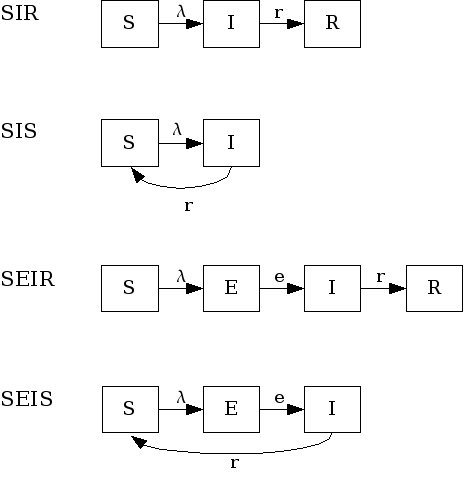
\includegraphics{SIRdiagram.png}
\caption{Figure: SIR-like models}\label{intromodels:fig-sir}\end{figure}

Variations of this model allow cases where infected individuals do not acquire immunity after infection, thus returning to the susceptible pool (\emph{SIS} model). Another variation is the inclusion of a latent stage to hold individuals that are infected but not infectious to others yet (incubation period). These are the \emph{SEIR} (with immunity) and \emph{SEIS} (no immunity) models.

Next, we describe in more detail each one of these models in their deterministic and stochastic versions, as used by EpiGrass.

\begin{tabulary}{\linewidth}{|c|l|}
\hline
\textsf{\relax 
\textbf{Symbol}
} & \textsf{\relax 
\textbf{Meaning}
}\\
\hline
\(L_t\)
 & 
number of newly infected individuals at time
\\

\(E\)
 & 
number of exposed but not infectious individuals
at time t
\\

\(I\)
 & 
number of infectious individuals at time t
\\

\(R\)
 & 
number of recovered individuals at time t
\\

\(\beta\)
 & 
contact rate (\(t^{-1}\))
\\

\(\theta\)
 & 
number of infectious visitors
\\

\(\alpha\)
 & 
mixing parameter (\(\alpha = 1\) means
homogeneous mixing)
\\

\(n\)
 & 
number of visitors
\\
 \multicolumn{2}{|l|}{
\(N\)      \textbar{} population \((S+E+I+R)\)
}\\
 \multicolumn{2}{|l|}{
\(B\)      \textbar{} susceptible pool replenishment
}\\

\(r\)
 & 
fraction of \(I\) recovering from infection
per unit of time \(([0,1])\)
\\

\(e\)
 & 
fraction of \(E\) becoming infectious per
unit of time \(([0,1])\)
\\

\(\delta\)
 & 
probability of acquiring immunity \(([0,1])\)
\\

\(w\)
 & 
probability of losing immunity \(([0,1])\)
\\

\(p\)
 & 
probability of recovered individual acquiring
infection, given exposure \(([0,1])\)
\\
\hline\end{tabulary}


\index{Models!SIR}\begin{description}
\item[{\textbf{SIR models}}] \leavevmode
Examples of diseases represented by SIR models are measles, chickenpox. Some diseases that do not confer lifelong immunity may be represented by this model if only short term dynamics is of interest. In the scale of a year, influenza and pertussis, for example, could be described using SIR. The SIR model is implemented in EpiGrass as a system of four difference equations. Besides the three equations describing the dynamics of \(S\), \(I\) and \(R\), a fourth equation explicitly defines the number of new cases per time step, \(L(t)\) (i.e., the incidence). In general, this quantity is embedded in the \(I\) equation (prevalence), but it is important to keep track of the incidence if one wishes to compare prediction with notification data.

\end{description}
\phantomsection\label{intromodels:equation-E:SIRmodel}\begin{align}
    L_{t+1} &= \beta S_t \frac{(I_t+\theta)^\alpha} {N_t+n_t}\nonumber \\
    I_{t+1} &= L_{t+1} + (1-r)I_t\nonumber\\
    S_{t+1} &= S_t + B - L_{t+1}\nonumber\\
    R_{t+1} &= N_t-(S_{t+1}+I_{t+1})\nonumber
\end{align}
This model can be easily extended to include diseases without recovery, for example AIDS, the so called SI models. Basically, the recovery rate is set to 0.

\index{Models!SIS}\begin{description}
\item[{\textbf{SIS models}}] \leavevmode
In the SIS model, individuals do not acquire immunity after the infection. They return directly to the susceptible class.

The only difference between \$SIS\$ and \$SIR\$ models is the absence of \$R\$ and the flow of recovered individuals to the susceptible stage:

\end{description}
\phantomsection\label{intromodels:equation-E:SISmodel}\begin{align}
        L_{t+1} &= \beta S_t \frac{(I_t+\theta)^\alpha} {N_t+n_t} \nonumber\\
        I_{t+1} &= L_{t+1} + (1-r)I_t\nonumber\\
        S_{t+1} &= S_t + B - L_{t+1} + r I_{t+1}\nonumber
\end{align}
\index{Models!SEIR}\begin{description}
\item[{\textbf{SEIR models}}] \leavevmode
These models have an extra compartment for those individuals who have acquired the infection but are still not infectious to others. This is the latent period and it is often parameterized as the inverse of the incubation period. Note, however, that for many diseases, initiation of infectiousness does not necessarily coincides with symptoms. In principle, any disease described by the SIR model can also be described by the SEIR model. The decision regarding the use of one or another depends on the magnitude of the latent period in relation to the time frame of other events in the simulation. The model has the form:

\end{description}
\phantomsection\label{intromodels:equation-E:SEIRmodel}\begin{align}
        L_{t+1} &= \beta S_t \frac{(I_t+\theta)^\alpha} {N_t+n_t}\nonumber \\
    E_{t+1} &= (1-e) E_t + L_{t+1}\nonumber\\
        I_{t+1} &= e E_t + (1-r)I_t\nonumber\\
        S_{t+1} &= S_t + B - L_{t+1}\nonumber\\
        R_{t+1} &= N_t-(S_{t+1}+I_{t+1}+E_{t+1})\nonumber
\end{align}
\index{Models!SEIS}\begin{description}
\item[{\textbf{SEIS models}}] \leavevmode
These are SIS models with the inclusion of the latent stage.

\end{description}
\phantomsection\label{intromodels:equation-E:SEISmodel}\begin{align}
        L_{t+1} &= \beta S_t \frac{(I_t+\theta)^\alpha} {N_t+n_t}\nonumber \\
    E_{t+1} &= (1-e) E_t + L_{t+1}\nonumber\\
        I_{t+1} &= e E_t + (1-r)I_t\nonumber\\
        S_{t+1} &= S_t + B - L_{t+1} + r I_t\nonumber
\end{align}

\subsubsection{SIpR-like models}
\label{intromodels:sipr-like-models}
These are \emph{SIR} models with immunity intermediary between full (\emph{SIR}) and null (\emph{SIS}).
Some possibilities arise here: 1) Infection confers full immunity to a fraction of the individuals and the remaining ones return to the susceptible class again, after infection. (\emph{SIpRpS}); 2) Infection provides only partial immunity and recovered individuals are partially susceptible to new infection (\emph{SIpR}); 3) Immunity is full right after infection but wanes with time (\emph{SIRS}). Each model is presented below. Figure \emph{fig:sipr} illustrates them diagrammatically.
\begin{figure}[htbp]
\centering
\capstart

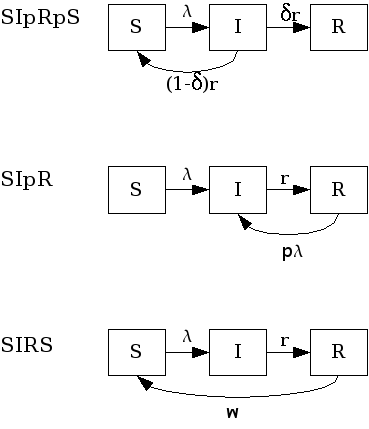
\includegraphics{SIpRdiagram.png}
\caption{SIpR-like models.}\end{figure}

Related models, that included the latent state \$E\$ are: textit\{SEIpRpS\}, \emph{SEIpR}, \emph{SEIRS}.

\index{Models!SIpRpS}\begin{description}
\item[{\textbf{SIpRpS model}}] \leavevmode
This model assumes that a fraction \$delta\$ of infectious individuals acquire full immunity while the remaining \$(1-delta)\$ returns to the susceptible stage. The model is:

\end{description}
\phantomsection\label{intromodels:equation-E:SIpRpSmodel}\begin{align}
        L_{t+1} &= \beta S_t \frac{(I_t+\theta)^\alpha} {N_t+n_t}\nonumber \\
        I_{t+1} &= L_{t+1} + (1-r)I_t\nonumber\\
        S_{t+1} &= S_t + B - L_{t+1} + (1-\delta) r I_t\nonumber\\
        R_{t+1} &= N_t-(S_{t+1}+I_{t+1})\nonumber
\end{align}\begin{description}
\item[{\textbf{SIpR model}}] \leavevmode
This model assumes that immunity is only partial and recovered individuals may acquire infection again (at a  lower rate \(p \lambda\), where \(0\leq p \leq 1\)). Two equations calculate the number of new infections. \(L_S\)  calculates the number of susceptibles that become infected at \(t+1\). \(L_R\)  calculates the number of recovered that become infected at \(t+1\). The latter are less susceptible to the disease when compared to susceptibles. The model is:

\end{description}
\phantomsection\label{intromodels:equation-E:SIpRmodel}\begin{align}
    L_{S,t+1} &= \beta S_t \frac{(I_t+\theta)^\alpha} {N_t+n_t}\nonumber \\
    L_{R,t+1} &= p \beta R_t \frac{(I_t+\theta)^\alpha} {N_t+n_t}\nonumber\\
    I_{t+1} &= L_{S,t+1} + L_{R,t+1} + (1-r)I_t\nonumber\\
    S_{t+1} &= S_t + B - L_{S,t+1} \nonumber\\
    R_{t+1} &= N_t-(S_{t+1}+I_{t+1}) \nonumber
    \end{align}
\index{Models!SIRS}\begin{description}
\item[{\textbf{SIRS model}}] \leavevmode
Here, the immunity acquired by infection wanes with time. Pertussis is an example of this dynamic.

\end{description}
\phantomsection\label{intromodels:equation-E:SIRSmodel}\begin{align} \label{}
        L_{S,t+1} &= \beta S_t \frac{(I_t+\theta)^\alpha} {N_t+n_t}\nonumber \\
    I_{t+1} &= L_{S,t+1} + L_{R,t+1} + (1-r)I_t\nonumber\\
        S_{t+1} &= S_t + B - L_{S,t+1} + w R_t\nonumber\\
        R_{t+1} &= N_t-(S_{t+1}+I_{t+1}) \nonumber
\end{align}

\subsubsection{SnInRn-like Models}
\label{intromodels:sninrn-like-models}
These are models with more than one compartment for susceptibles,
infected and recovered stages. They are used when infection involves
more than one distinct populations. Vector borne diseases are
classical examples where a SIR model is used to describe infection in
humans and another SIR-like model is used to describe infection in the
vector (and/or the reservoir(s)). Dengue fever and yellow fever are
examples. Sexually transmitted diseases may also be modeled with
SnInRn models if male and female populations are distinguished. These
models can be define by the user as a custom model.


\subsection{Stochastic models}
\label{intromodels:stochastic-models}
\index{Models!Stochastic}
All models described so far are deterministic. EpiGrass allows simulation of stochastic processes. This is done by assuming that \(L_{t+1}\) is a random variable with expected value given by the expressions found in the deterministic models. The user may choose the probability distribution for \(L_{t+1}\) between Poisson or Negative Binomial to draw realizations of \(L_{t+1}\):
\begin{gather}
\begin{split}l_{t+1} \sim Poisson (L_{t+1})\end{split}\notag
\end{gather}
or
\begin{gather}
\begin{split}l_{t+1} \sim NegBin (I_t, \frac{I_t}{I_t+L_{t+1}})\end{split}\notag
\end{gather}
The Poisson distribution assumes independent events while the negative Binomial assume clustering of transmission events.


\section{Network transportation models}
\label{intromodels:network-transportation-models}
\index{Models!transportation}
The transmission models describe the dynamics of infection in a well-mixed population. EpiGrass allows the user to model the movement of infectious individuals between well-mixed populations, thus simulating the spread of disease through space. EpiGrass represents geographical space as a network where cities or localities are nodes and transportation routes are edges. The term network refers to the framework of routes within a system of locations, identified as nodes or sites. An edge is a single link between two sites (a road, a railroad, an air route or a river/sea corridor).

Transportation networks, like many networks, are generally embodied as
set of locations and a set of links representing connections between
those locations. The arrangement and connectivity of a network is
known as its \emph{topology}. Major types of topology are
illustrated in figure ref\{fig:artgraphs\}. Velocity and direction of
disease spread depend on the topology and weight of the edges of the
transport network and there are many properties of networks that may
useful when analyzing the spread of diseases. EpiGrass calculates a
set of these properties as described in chapter {\hyperref[analysis:analysis]{\emph{Analysis}}}.

In a transportation network, each edge (or link) is characterized by a variable \emph{flow} which states the number of passengers that travel through that link per unit time. EpiGrass uses this information to calculate the number of passengers arriving at each city, per time step. For example, consider node \(N1\) in figure {\hyperref[intromodels:simpnet]{\emph{A simple transportation network}}}. At each time step, it receives 10 passengers from \(N2\), 5 from \(N5\), 1 from \(N4\). Now suppose that, at this time step, 10\% of the population within each site is infectious (\(I\) state), according to the epidemic model. Thus, a total of \(10\% \times 10 + 10\% \times 5 + 10\% \times 1 = 1.6\) infectious individuals are visiting site \(N1\). In the epidemic model embedded in \(N1\), EpiGrass sets \(n = 16\) and \(\theta = 1.6\). This calculation of \(\theta\) is based on a deterministic argument. The other possibility, allowed by Epigrass, is to define \(\theta\) as a random variable, that follows a binomial distribution with parameters \(n\),:math:\emph{p}, where \(n\) is as given in the deterministic version and \(p\) is the proportion of infectious individuals in the source population. From version 1.4 on, EpiGrass can also take into account the specific delays of each connection. When the average speed of the transportation system is set to a value greater than zero, epigrass calculates the time required to complete each trip and attributes this delay (in units of time) to the parameter \(\delta\). So, the number of infectious passengers arriving at any given city, at time \(t\) corresponds to the number of infectious passengers that left the city of origin at time \(t-\delta\).

Deterministic:
\begin{gather}
\begin{split}\Theta_t=n\times\frac{I_{t-\delta}}{N}\end{split}\notag
\end{gather}
Stochastic:
\begin{gather}
\begin{split}\Theta_t \sim Binomial(N,\frac{I_{t-\delta}}{N})\end{split}\notag
\end{gather}\begin{figure}[htbp]
\centering
\capstart

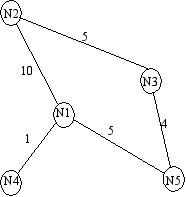
\includegraphics{simplenet.png}
\caption{A simple transportation network}\label{intromodels:simpnet}\end{figure}


\chapter{Using Epigrass}
\label{using::doc}\label{using:using}\label{using:using-epigrass}
To simulate an epidemic process in Epigrass, the user needs to have in hand at least three files: Two files containing the site and edge data and a third file which is a script that defines what it is to be done. Here we go through each one of them in detail. The last part of this chapter is a step-by step guide the Graphical User Interface (GUI).


\section{Data}
\label{using:data}

\subsection{Site data file}
\label{using:site-data-file}
See below an example of the content of a site file for a network of 10 cities. Each line corresponds to a site (except the first line which is the title). For each site, it is declared, in this order: its \emph{spatial location} in the form of a pair of coordinates ({[}X,Y{]}); a site \$name\$ to be used in the output; the site's population; the site geocode (an arbitrary unique number which is used internally by Epigrass).

\begin{tabulary}{\linewidth}{|l|c|c|c|c|}
\hline
\textsf{\relax 
X
} & \textsf{\relax 
Y
} & \textsf{\relax 
City
} & \textsf{\relax 
Pop
} & \textsf{\relax 
Geocode
}\\
\hline
1
 & 
4
 & 
``N1''
 & 
1000000
 & 
1
\\

2
 & 
4
 & 
``N2''
 & 
100000
 & 
2
\\

3
 & 
4
 & 
``N3''
 & 
1000
 & 
3
\\

4
 & 
4
 & 
``N4''
 & 
1000
 & 
4
\\

5
 & 
4
 & 
``N5''
 & 
1000
 & 
5
\\

1
 & 
3
 & 
``N6''
 & 
100000
 & 
6
\\

2
 & 
3
 & 
``N7''
 & 
1000
 & 
7
\\

3
 & 
3
 & 
``N8''
 & 
100000
 & 
8
\\

4
 & 
3
 & 
``N9''
 & 
100000
 & 
9
\\

5
 & 
3
 & 
``N10''
 & 
1000
 & 
10
\\

1
 & 
2
 & 
``N11''
 & 
1000
 & 
11
\\
\hline\end{tabulary}


In this example, the first site is located at \emph{{[}X,Y{]}={[}1,4{]}}, it is named N1, its population is 1000000 and its geocode is 1. This is minimum configuration of a site data file and it must contains this information in exactly this order.

In some situations, the user may want to add other attributes to the sites (different transmission parameters, or vaccine coverage or initial conditions for simulations). This information is provided by adding new columns to the minimum file. For example, if one wishes to add information on the vaccine coverage in cities N1 to N10 (\$vac\$) as well as information about average temperature (which hypothetically affects the transmission of the disease), the file becomes:

\begin{tabulary}{\linewidth}{|L|L|L|L|L|L|L|}
\hline
\textsf{\relax 
X
} & \textsf{\relax 
Y
} & \textsf{\relax 
City
} & \textsf{\relax 
Pop
} & \textsf{\relax 
Geocode
} & \textsf{\relax 
Vac
} & \textsf{\relax 
Temp
}\\
\hline
1
 & 
4
 & 
``N1''
 & 
1000000
 & 
1
 & 
0.9
 & 
32
\\

2
 & 
4
 & 
``N2''
 & 
100000
 & 
2
 & 
0.88
 & 
29
\\

3
 & 
4
 & 
``N3''
 & 
1000
 & 
3
 & 
0.7
 & 
25
\\

4
 & 
4
 & 
``N4''
 & 
1000
 & 
4
 & 
0.2
 & 
34
\\

5
 & 
4
 & 
``N5''
 & 
1000
 & 
5
 & 
0
 & 
26
\\

1
 & 
3
 & 
``N6''
 & 
100000
 & 
6
 & 
0
 & 
27
\\

2
 & 
3
 & 
``N7''
 & 
1000
 & 
7
 & 
0
 & 
31
\\

3
 & 
3
 & 
``N8''
 & 
100000
 & 
8
 & 
0
 & 
30
\\

4
 & 
3
 & 
``N9''
 & 
100000
 & 
9
 & 
0
 & 
24
\\

5
 & 
3
 & 
``N10''
 & 
1000
 & 
10
 & 
0
 & 
31
\\
\hline\end{tabulary}


During the simulation, each site object receives these informations and store them in appropriate variables that can be used later during model specification. Population is stored in the variable  \emph{N}; while the extra columns (those beyond the geocode) are stored in a tuple named \emph{\{values}. For example, for the city  \emph{N1}, we have  \emph{N = 1000000} and  \emph{values={[}0.9,32{]}}. During model specification, we may use  \emph{N} to indicate the population size and/or we can use \emph{values{[}0{]}} to indicate the level of vaccination of that city and \emph{values{[}1{]}} to indicate the temperature.

It is up to the user, to know what means the elements of the tuple \emph{values}. Note that the first element of the tuple has index 0,the second one has index 1 and so on.

When using real data, one may wish to use actual geocodes and coordinates. For example, for a network of Brazilian cities, one may build the following file:

\begin{tabulary}{\linewidth}{|L|L|L|L|L|}
\hline
\textsf{\relax 
latitude
} & \textsf{\relax 
longitude
} & \textsf{\relax 
local
} & \textsf{\relax 
pop
} & \textsf{\relax 
geocode
}\\
\hline
-16:19:41
 & 
-48:57:10
 & 
ANAPOLIS
 & 
280164
 & 
520110805
\\

-10:54:32
 & 
-37:04:03
 & 
ARACAJU
 & 
461534
 & 
280030805
\\

-21:12:27
 & 
-50:26:24
 & 
ARACATUBA
 & 
164449
 & 
350280405
\\

-18:38:44
 & 
-48:11:36
 & 
ARAGUARI
 & 
92748
 & 
310350405
\\

-21:13:17
 & 
-43:46:12
 & 
BARBACENA
 & 
103669
 & 
310560805
\\

-22:32:53
 & 
-44:10:30
 & 
BARRA\_MANSA
 & 
165134
 & 
330040705
\\

-20:33:11
 & 
-48:34:11
 & 
BARRETOS
 & 
98860
 & 
350550005
\\

-26:54:55
 & 
-49:04:15
 & 
BLUMENAU
 & 
241943
 & 
420240405
\\

-22:57:09
 & 
-46:32:30
 & 
B.PAULISTA
 & 
111091
 & 
350760505
\\
\hline\end{tabulary}


In this file, the coordinates are the actual geographical latitude and longitude coordinates. This information is important when using Epigrass with a map in shapefile format. The geocode is also the official geocode of these localities (the same one used in the shapefile). Despite the cumbersome size of the number, it may be worth using it because demographic official databases are often linked by this number.


\subsection{Edge data file}
\label{using:edge-data-file}
The edge data file contains all the direct links between sites. Each line in the file (except for the first, which is the header) corresponds to an edge. For each edge (or link) one must specify (in this order): the \emph{names of the sites} connected by that edge; the \emph{number of individuals traveling from source to destination}; the \emph{number of individuals travelling from destination to source} per time step; the \emph{distance or length} of the edge. At last, the file must contain, in the fifth and sixth columns, the \emph{geocodes} of the source and destination sites*. This is very important as the graph is built internally connecting sites through edges and this is done based on geocode info.

\begin{notice}{warning}{Warning:}
It is required that the order of columns is kept the same.
\end{notice}

See below the list of the 8 edges connecting the sites \emph{N1} to \emph{N10}. Let's look the first one, as an example. It links \emph{N1} to \emph{N2}. Through this link passes 11 individuals backwards and forwards per time step (a day, for example). This edge has length 1 (remember that \emph{N1} is at {[}X,Y{]}={[}1,1{]} and \emph{N2} is at {[}X,Y{]}={[}1,2{]}, so the distance between them is 1). The last two columns show the geocode of \emph{N1} (geocode 1) and the geocode of \emph{N2} (geocode 2).

\begin{tabulary}{\linewidth}{|L|L|L|L|L|L|L|}
\hline
\textsf{\relax 
Source
} & \textsf{\relax 
Dest
} & \textsf{\relax 
flowSD
} & \textsf{\relax 
flowDS
} & \textsf{\relax 
Distance
} & \textsf{\relax 
geoSource
} & \textsf{\relax 
geoDest
}\\
\hline
N1
 & 
N2
 & 
11
 & 
11
 & 
1
 & 
1
 & 
2
\\

N2
 & 
N4
 & 
0.02
 & 
0.02
 & 
1
 & 
3
 & 
4
\\

N3
 & 
N8
 & 
1.01
 & 
1.01
 & 
1
 & 
3
 & 
8
\\

N4
 & 
N9
 & 
1.01
 & 
1.01
 & 
1
 & 
4
 & 
9
\\

N5
 & 
N10
 & 
0.02
 & 
0.02
 & 
1
 & 
5
 & 
10
\\

N6
 & 
N5
 & 
1.01
 & 
1.01
 & 
1
 & 
7
 & 
8
\\

N7
 & 
N10
 & 
1.01
 & 
1.01
 & 
1
 & 
7
 & 
8
\\

N9
 & 
N10
 & 
1.01
 & 
1.01
 & 
1
 & 
9
 & 
10
\\
\hline\end{tabulary}


Note that it doesn't matter which site is considered a Source and which one is considered a Destination. I.e., if there is a link between \emph{A} and \emph{B}, one may either named \emph{A} as source and \emph{B} as destination, or the other way around.

If the edge represents a road or a river, one may use the actual metric distance as length. If the edge links arbitrary localities, one may opt to use euclidean distance, calculated from the \emph{x} and \emph{y} coordinates (using Pythagoras theorem).


\section{Specifying a model: the script}
\label{using:specifying-a-model-the-script}
Once the user has specified the two data files, the next step is to define the model to be executed. This is done in the .epg script file. The   \code{.epg} script is a text file and can be edited with any editor (not word processor). This script must be prepared with care.

The best way to write down your own .epg is to edit an already existing .epg file. So, open Epigrass, choose an .epg file and click on the \emph{Edit} button. Your favorite editor will open and you can start editing. Don't forget to save it as a new file in your working directory. Of course, there is an infinite number of possibilities regarding the elaboration of the script. It all depends on the goals of the user.

\begin{notice}{note}{Note:}
Another way to edit an .epg file is to open it whith the graphical editor provided with Epigrass. Just type \code{epgeditor yourmodel.epg}.
\end{notice}

For the beginner, we suggest him/her to take a look at the .epg files in the demo directory. They are all commented and may help the user in getting used with Epigrass language and capabilities.

Some hints to be successful when editing your   \code{.epg}:
\begin{itemize}
\item {} 
All comments in the script are preceded by the symbol \#. These comments may be edited by the user as he/she wishes and new lines may be added at will. Don't forget, however, to place the symbol \# in every line corresponding to a comment.

\item {} 
The script is divided into a few parts. These parts have capital letter titles within brackets. Don't touch them!

\item {} 
Don't remove any line that is \emph{not} a comment. See below how to appropriately edit these command lines.

\end{itemize}

Let's take a look now at each part of a script (this is the script  \code{.epg} demo file):

\begin{notice}{warning}{Warning:}
All variables defined in a \code{.epg} are \textbf{case-insensitive}. Consider this fact when naming your model's variables.
\end{notice}


\subsection{Part 1: THE WORLD}
\label{using:part-1-the-world}
The first section of the script is titled: THE WORLD. An example of its content is shown:

\begin{Verbatim}[commandchars=\\\{\}]
shapefile = [\PYGZsq{}riozonas\PYGZus{}LatLong.shp\PYGZsq{},\PYGZsq{}nome\PYGZus{}zonas\PYGZsq{},\PYGZsq{}zona\PYGZus{}trafe\PYGZsq{}]
edges = edges.csv
sites = sites.csv
encoding =
\end{Verbatim}

where,
\begin{description}
\item[{\textbf{shapefile}}] \leavevmode
Is a list with 3 elements: the first is  the path, relative to the working directory, of the shapefile file; the second  is the variable, in the shapefile, which contains the names of the localities (polygons of the map); the third and last is the variable, in the shapefile, which contains the geocode of the localities. If you don't have a map for you simulation, leave the list empty: \emph{location = {[}{]}} ).

\item[{\textbf{edges}}] \leavevmode
This is the name of the .CSV (comma-separated-values) file containing the list of edges and their attributes.

\item[{\textbf{sites}}] \leavevmode
This is the name of the .CSV file containing the list of sites and their attributes.

\item[{\textbf{encoding}}] \leavevmode
This is the encoding used in your sites and edges files. This is very important when you use location names which include non-ascii characters. The default encoding is \emph{latin-1}. If you use any other encoding, please specify it here. Example: \emph{utf-8}.

\end{description}

\begin{notice}{note}{Note:}
All paths in the \code{.epg} file are relative to the working directory.
\end{notice}


\subsection{Part 2: EPIDEMIOLOGICAL MODEL}
\label{using:part-2-epidemiological-model}
This is the main part of the script. It defines the epidemiological model to be run.
The script reads:

\begin{Verbatim}[commandchars=\\\{\}]
\PYG{n}{modtype} \PYG{o}{=} \PYG{n}{SIR}
\end{Verbatim}

Here, the type of epidemiological model is defined, in this case is a deterministic \emph{SIR} model. Epigrass has some built-in models:

\begin{tabulary}{\linewidth}{|L|L|L|}
\hline
\textsf{\relax 
Name
} & \textsf{\relax 
Determ.
} & \textsf{\relax 
Stochastic
}\\
\hline
Susceptible-Infected-Recovered
 & 
\emph{SIR}
 & 
\emph{SIR\_s}
\\

Susceptible-Exposed-Infected-Recovered
 & 
\emph{SEIR}
 & 
\emph{SEIR\_s}
\\

Susceptible-Infected-Susceptible
 & 
\emph{SIS}
 & 
\emph{SIS\_s}
\\

Susceptible-Exposed-Infected-Susceptible
 & 
\emph{SEIS}
 & 
\emph{SEIS\_s}
\\

SIR with fraction with full immunity
 & 
\emph{SIpRpS}
 & 
\emph{SIpRpS\_s}
\\

SEIR with fraction with full immunity
 & 
\emph{SEIpRpS}
 & 
\emph{SEIpRpS\_s}
\\

SIR with partial immunity for all
 & 
\emph{SIpR}
 & 
\emph{SIpR\_s}
\\

SEIR with partial immunity for all
 & 
\emph{SEIpR}
 & 
\emph{SEIpR\_s}
\\

SIR with immunity wane
 & 
\emph{SIRS}
 & 
\emph{SIRS\_s}
\\
\hline\end{tabulary}


A description of these models can be found in the chapter \emph{Epidemiological modeling}. The stochastic models use \emph{Poisson} distribution as default for the number of new cases (\emph{L(t+1)}). Besides these, the user may define his/her own model and access by the protect word Custom.


\subsection{Part 3: MODEL PARAMETERS}
\label{using:part-3-model-parameters}
The epidemic model is defined by variables and parameter which require initialization:

\begin{Verbatim}[commandchars=\\\{\}]
\PYG{c}{\PYGZsh{}==============================================================\PYGZsh{}}
    \PYG{c}{\PYGZsh{}  They can be specified as constants or as functions of global or}
    \PYG{c}{\PYGZsh{}  site\PYGZhy{}specific variables. Site\PYGZhy{}specific variables are provided}
    \PYG{c}{\PYGZsh{}  in the sites .csv file. In this file, all columns after the 4th}
    \PYG{c}{\PYGZsh{}  are collected into a values tuple, which can be referenced here}
    \PYG{c}{\PYGZsh{}  as values[0], values[1], values[2], etc.}
    \PYG{c}{\PYGZsh{}   Examples:}
    \PYG{c}{\PYGZsh{}   beta = 0.001}
    \PYG{c}{\PYGZsh{}   beta=values[0] \PYGZsh{}assigns the first element of values to beta}
    \PYG{c}{\PYGZsh{}   beta=0.001*values[1]}
    \PYG{c}{\PYGZsh{}   beta=0.001*N  \PYGZsh{} N is a global name for total site population}
    \PYG{c}{\PYGZsh{} Currently, Epigrass requires that parameters beta, alpha, e, r, delta, B, w, p}
    \PYG{c}{\PYGZsh{} be present in the .epg even if they will not be used. Do not erase these lines.}
    \PYG{c}{\PYGZsh{} Just disregard them if they are not useful to you.}

\PYG{n}{beta} \PYG{o}{=} \PYG{l+m+mf}{0.4}   \PYG{c}{\PYGZsh{}transmission coefficient (contact rate * transmissibility)}
\PYG{n}{alpha} \PYG{o}{=} \PYG{l+m+mi}{1}  \PYG{c}{\PYGZsh{} clumping parameter}
\PYG{n}{e} \PYG{o}{=} \PYG{l+m+mi}{1}   \PYG{c}{\PYGZsh{} inverse of incubation period}
\PYG{n}{r} \PYG{o}{=} \PYG{l+m+mf}{0.1}   \PYG{c}{\PYGZsh{} inverse of infectious period}
\PYG{n}{delta} \PYG{o}{=} \PYG{l+m+mi}{1}  \PYG{c}{\PYGZsh{} probability of acquiring full immunity [0,1]}
\PYG{n}{B} \PYG{o}{=} \PYG{l+m+mi}{0}           \PYG{c}{\PYGZsh{} Birth rate}
\PYG{n}{w} \PYG{o}{=} \PYG{l+m+mi}{0}           \PYG{c}{\PYGZsh{} probability of immunity waning [0,1]}
\PYG{n}{p} \PYG{o}{=} \PYG{l+m+mi}{0}           \PYG{c}{\PYGZsh{}}
\end{Verbatim}

These are the model parameters. Not all parameters are necessary for all models. For example, \emph{e} is only required for SEIR-like models. Don't
remove the line, however because that will cause an error. We recommend that, if the parameter is not necessary, just add a comment after it as a reminder that it is not being used by the model.

In some cases, one may wish to assign site-specific parameters. For example, transmission rate may be different between localities that are very distant and are exposed to different climate. In this case site specific variables can be added as new columns to the site file. All columns after the geocode are packed into a tuple named \emph{values} and can be referenced in the order they appear. I.e., the first element of the tuple is \emph{values{[}0{]}}, the second element is \emph{values{[}1{]}}, the third element is \emph{values{[}2{]}} and so on.

Part 4: INITIAL CONDITIONS

In this part of the script, the initial conditions are defined. Here, the number of individuals in each epidemiological state, at the start of the simulation, is specified. It reads:

\begin{Verbatim}[commandchars=\\\{\}]
\PYG{c}{\PYGZsh{}==============================================================\PYGZsh{}}
\PYG{c}{\PYGZsh{} Here, the number of individuals in each epidemiological}
\PYG{c}{\PYGZsh{} state (SEI) is specified. They can be specified in absolute}
\PYG{c}{\PYGZsh{} or relative numbers.}
\PYG{c}{\PYGZsh{} N is the population size of each site.}
\PYG{c}{\PYGZsh{} The rule defined here will be applied equally to all sites.}
\PYG{c}{\PYGZsh{} For site\PYGZhy{}specific definitions, use EVENTS (below)}
\PYG{c}{\PYGZsh{} Examples:}
\PYG{c}{\PYGZsh{}   S,E,I = 0.8*N, 10, 0.5*N}
\PYG{c}{\PYGZsh{}   S,E,I = 0.5*N, 0.01*N, 0.05*N}
\PYG{c}{\PYGZsh{}   S,E,I = N\PYGZhy{}1, 1, 0}
\PYG{n}{S} \PYG{o}{=} \PYG{n}{N}
\PYG{n}{E} \PYG{o}{=} \PYG{l+m+mi}{0}
\PYG{n}{I} \PYG{o}{=} \PYG{l+m+mi}{0}
\end{Verbatim}

Here, \emph{N} is the total population in a site (as in the datafile for sites). In this example, we set all localities to the same initial conditions (all individuals susceptible) and use an event (see below) to introduce an infectious individual in a locality. The number of recovered individuals is implicit, as \emph{R = N-(S+E+I)}

Another possibility is to define initial conditions that are different for each site. For this, the data must be available as extra columns in the site data file and these columns are referenced to using the \emph{values} tuple explained above.


\subsection{Part 5: EPIDEMIC EVENTS}
\label{using:part-5-epidemic-events}
The next step is to define events that will occur during the simulation. These events may be epidemiological (arrival of an infected, for example) or a public health action (vaccination campaign, for example):

\begin{Verbatim}[commandchars=\\\{\}]
\PYG{c}{\PYGZsh{}=============================================================\PYGZsh{}}
\PYG{c}{\PYGZsh{}   Specify isolated events.}
\PYG{c}{\PYGZsh{}   Localities where the events are to take place should be Identified by the geocode, which}
\PYG{c}{\PYGZsh{}  comes after population size on the sites data file.}
\PYG{c}{\PYGZsh{}  All coverages must be a number between 0 and 1.}
\PYG{c}{\PYGZsh{}  Seed : [(\PYGZsq{}locality1\PYGZsq{}s geocode\PYGZsq{},epid state, n),(\PYGZsq{}locality2\PYGZsq{}s geocode\PYGZsq{}, epid state, n),...]}
\PYG{c}{\PYGZsh{}  N infected cases will be added to locality at time 0.}
\PYG{c}{\PYGZsh{}  Vaccinate: [(\PYGZsq{}locality1\PYGZsq{}s geocode\PYGZsq{}, [t1,t2,...], [cov1,cov2,...]),(\PYGZsq{}locality2\PYGZsq{}s geocode\PYGZsq{}, [t1,t2,...], [cov1,cov2,...])]}
\PYG{c}{\PYGZsh{}  Quarantine: [(locality1\PYGZsq{}s geocode,time,coverage), (locality2\PYGZsq{}s geocode,time,coverage)]}
\PYG{c}{\PYGZsh{}seed = [(4550601,\PYGZsq{}ip20\PYGZsq{},10)] \PYGZsh{}santo cristo  \PYGZsh{}}
\PYG{n}{seed} \PYG{o}{=} \PYG{p}{[}\PYG{p}{(}\PYG{l+m+mi}{4552110}\PYG{p}{,}\PYG{l+s}{\PYGZsq{}}\PYG{l+s}{ip20}\PYG{l+s}{\PYGZsq{}}\PYG{p}{,}\PYG{l+m+mi}{10}\PYG{p}{)}\PYG{p}{]} \PYG{c}{\PYGZsh{}pechincha  \PYGZsh{}}
\PYG{c}{\PYGZsh{}seed = []}
\PYG{n}{Vaccinate} \PYG{o}{=} \PYG{p}{[}\PYG{p}{]} \PYG{c}{\PYGZsh{}}
\PYG{n}{Quarantine} \PYG{o}{=} \PYG{p}{[}\PYG{p}{]}
\end{Verbatim}

The events currently implemented are:
\begin{description}
\item[{\textbf{seed}}] \leavevmode
One or more infected individual(s) are introduced into a site, at the beggining of the simulation. The notation for a single event is: \emph{Seed = {[}(`locality1's geocode',epid state, n),(`locality2's geocode', epid state, n),...{]}}. For example, \emph{seed = {[}(2,'I',10){]}} programs the arrival of 10 infected individuals at site geocode 2, at time 1.

\item[{\textbf{Vaccinate}}] \leavevmode
Implements a campaign that vaccinates a fraction of the population in a site, at a pre-defined time-step. For multiple events, the notation is: \emph{{[}(`locality1's geocode', {[}t1,t2,...{]}, {[}cov1,cov2,...{]}),(`locality2's geocode', {[}t1,t2,...{]}, {[}cov1,cov2,...{]}){]}}, where the first element of every triplet is the geocode of the city, the second element is a list of the time(s) when the campaign is carried on, and the third element is the coverage(s). For example, the event \emph{{[}(2,{[}10{]},{[}0.7{]}){]}} means that city 2, at time 10, has 70\% of its population vaccinated. Mathematically, it means (in the model), the removal of individuals from the susceptible to the recovered stage.

\item[{\textbf{Quarantine}}] \leavevmode
Prevents any individual from leaving a site, starting at \emph{t}. Currently disabled.

\end{description}


\subsection{Part 6: TRANSPORTATION MODEL}
\label{using:part-6-transportation-model}
Here, there are two options regarding the movement of infected individuals from site to site (through the edges). If \emph{stochastic = 0}, the process is simulated deterministically. The number of infected passengers commuting through an edge is a fraction \emph{p} of the infected population that is traveling. \emph{p} is calculated as \emph{total passengers/total population}.

If \emph{stochastic = 1}, the number of passengers is sampled from a Poisson distribution with parameter given by the expected number of travelling infectives (calculated as above):

\begin{Verbatim}[commandchars=\\\{\}]
\PYG{c}{\PYGZsh{}=========================================================\PYGZsh{}}
\PYG{c}{\PYGZsh{} If doTransp = 1 the transportation dynamics will be}
\PYG{c}{\PYGZsh{} included. Use 0 here only for debugging purposes.}
\PYG{n}{doTransp} \PYG{o}{=} \PYG{l+m+mi}{1}

\PYG{c}{\PYGZsh{} Mechanism can be stochatic (1) or deterministic(0).}
\PYG{n}{stochastic} \PYG{o}{=} \PYG{l+m+mi}{1}
\PYG{c}{\PYGZsh{}Average speed of transportation system in km per time step. Enter 0 for instantaneous travel.}
\PYG{c}{\PYGZsh{}Distance unit must be the same specified in edges files}
\PYG{n}{speed} \PYG{o}{=}\PYG{l+m+mi}{0} \PYG{c}{\PYGZsh{}1440  km/day \PYGZhy{}\PYGZhy{} equivalent to 60 km/h}
\end{Verbatim}

That ends the definition of the model.


\subsection{Part 7: SIMULATION AND OUTPUT}
\label{using:part-7-simulation-and-output}
Now it is time to define some final operational variables for the simulation:

\begin{Verbatim}[commandchars=\\\{\}]
\PYGZsh{}==============================================================\PYGZsh{}
\PYGZsh{} Number of steps
steps = 50

\PYGZsh{} Output dir. Must be a full path. If empty the output will be generated on the
\PYGZsh{} same path as the model script.
outdir =

\PYGZsh{} Output file
outfile = simul.dat

\PYGZsh{} Database Output
\PYGZsh{} MySQLout can be 0 (no database output) or 1
MySQLout = 1


\PYGZsh{} Report Generation
\PYGZsh{} The variable report can take the following values:
\PYGZsh{} 0 \PYGZhy{} No report is generated.
\PYGZsh{} 1 \PYGZhy{} A network analysis report is generated in PDF Format.
\PYGZsh{} 2 \PYGZhy{} An epidemiological report is generated in PDF Format.
\PYGZsh{} 3 \PYGZhy{} A full report is generated in PDF Format.
\PYGZsh{} siteRep is a list with site geocodes. For each site in this list, a detailed report is apended to the main report.
report = 0
siteRep = []

\PYGZsh{} Replicate runs
\PYGZsh{} If replicas is set to an integer(n) larger than zero, the model will be run
\PYGZsh{} n times and the results will be consolidated before storing.
\PYGZsh{} RandSeed = 1: the seed will be randomized on each replicate
\PYGZsh{} RandSeed = 2: seeds are taken sequentially from the site\PYGZsq{}s file
\PYGZsh{} Note: Replicate mode automatically turn off report and batch options.
Replicas = 10
RandSeed = 2
\PYGZsh{}Batch Run
\PYGZsh{}  list other scripts to be run in after this one. don\PYGZsq{}t forget the extension .epg
\PYGZsh{}  model scripts must be in the same directory as this file or provide full path.
\PYGZsh{}  Example: Batch = [\PYGZsq{}model2.epg\PYGZsq{},\PYGZsq{}model3.epg\PYGZsq{},\PYGZsq{}/home/jose/model4.epg\PYGZsq{}]
Batch = []\PYGZsh{}[\PYGZsq{}sarsDF.epg\PYGZsq{},\PYGZsq{}sarsPA.epg\PYGZsq{},\PYGZsq{}sarsRS.epg\PYGZsq{}]
\end{Verbatim}

where,
\begin{description}
\item[{\textbf{step}}] \leavevmode
Number of time steps for the simulation.

\item[{\textbf{outdir}}] \leavevmode
Directory for data output (currently not in use)

\item[{\textbf{outfile}}] \leavevmode
.csv filename that can be imported into R as a dataframe. This .csv file contains the simulated timeseries for all nodes.

\item[{\textbf{MySQLout}}] \leavevmode
Use \emph{MySQLout = 1} if simulated time series are to be stored in MySQL database. Time series of \emph{L}, \emph{S}, \emph{E}, and \emph{I}, from simulations, are stored in a MySQL database named \emph{epigrass}. The results of each individual simulation is stored in a different table named after the model's script name, the date and time the simulation has been run. For instance, suppose you run a simulation of a model stored in a file named \code{script.epg}, then at the end of the simulation, a new table in the epigrass database will be created with the following name: \emph{script\_Wed\_Jan\_26\_154411\_2005}. Thus, the results of multiple runs from the same model get stored independently.

\item[{\textbf{Batch={[}{]}}}] \leavevmode
Script files included in this list are executed after the currently file is finished.

\end{description}


\section{The Graphical User Interface(GUI)}
\label{using:the-graphical-user-interface-gui}
Epigrass comes with a simple but effective GUI, that allows the user to control some aspects of the run-time behavior of the system. The Gui can be invoked by typing texttt\{epigrass\} in prompt of a console. We suggest the user to start Epigrass from the same directory where his/her model definition is located (\code{.csv} and   \code{.epg} files).

All the information that is entered via the GUI gets  stored in a hidden file called texttt\{.epigrassrc\} stored in the home folder of the user. Every time the GUI is invoked, the data stored in the texttt\{.epigrassrc\} file is used to fill the forms in the GUI. The gui is designed as a tabbed notebook with four tabs (Run Options, Settings, Utilities, and Visualization).

At the bottom of the Gui there are three buttons \emph{Help}, \emph{Start} and \emph{Exit}. Their functions will be explained below. Immediately above the \emph{Run} and \emph{Exit} buttons, there is a small numeric display that will display the simulation progress after it has been started.
\begin{figure}[htbp]
\centering
\capstart

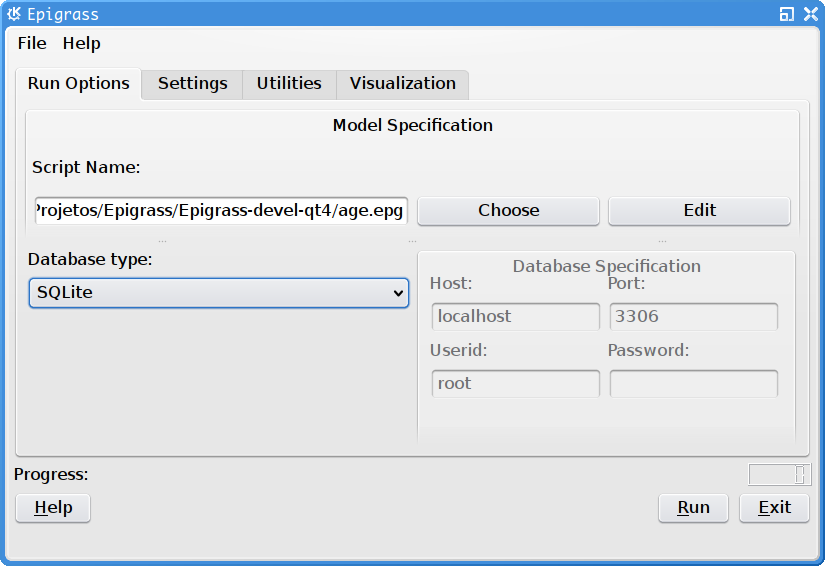
\includegraphics{epigrass1.png}
\caption{First tab of Epigrass GUI. This is where you setup your database output settings and the model to be run.}\end{figure}


\subsection{Run Options}
\label{using:run-options}
The first tab of the GUI, contains a number of variables that, with the exception of the model script filename, should remain the same for most simulations you are going to run.

On the top of the first tab is a text box to enter the file name of the model script (\code{something.epg}). By clicking on the \emph{Choose} button at the right of this box, you get a file selection dialog to select your script file. If you need you can click on the \emph{Edit} button below to edit the script file with your favorite text editor.

Below, you can enter details about the MySQL database that will store the output of your simulations. Here you can enter the server IP, port, user and password. On the first time you run the GUI these input boxes will be filled with the default values for these variables (server on localhost, port 3306, user epigrass and password epigrass)


\subsection{Settings}
\label{using:settings}
On the settings page, you can enter personal details such as user name (To be used in the simulation report), preferred text editor and preferred PDF reader. The preferred text editor will be used to open your script from the GUI, when you click on the edit button in the first tab. The PDF reader specified, will be used to open the report file, when requested (Utilities tab) and the user manual, when the user clicks on the help button on the bottom-left corner of the GUI.

On this tab, the language of the GUI can also be selected from a list of available translations. The effects of language changes will only take place when the next time the GUI is started.
\begin{figure}[htbp]
\centering
\capstart

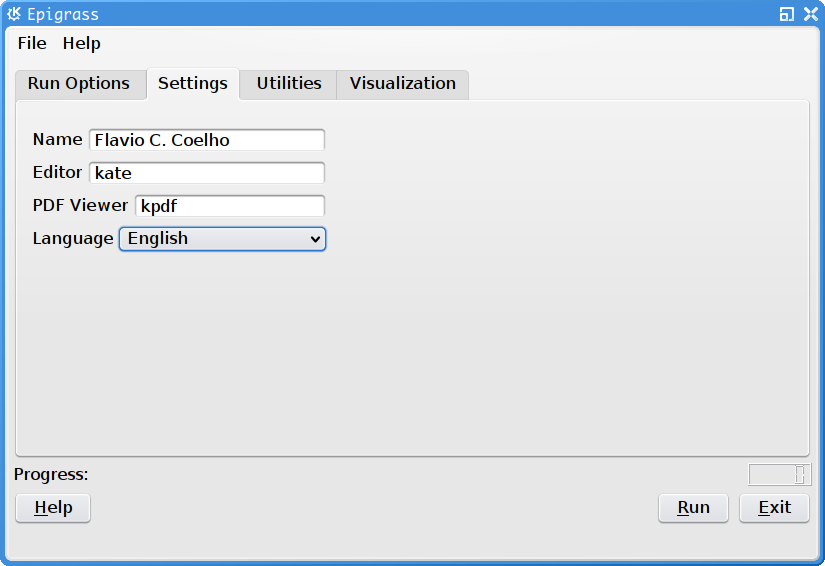
\includegraphics{epigrass2.png}
\caption{Settings tab of the Epigrass GUI. This is wher you configure the behavior os the GUI. Values set here will be remembered on future runs.}\end{figure}


\subsection{Utilities}
\label{using:utilities}
In the Utilities tab, you can get feed back from the simulator. Especially during long simulation runs, it is good to know how it is progressing. During the simulation, text messages regarding the status of the simulation are written to the text box on the left.

On the right, there is a button for backing up the data base and another for opening the report generated by the last simulation. Since report PDFs ar stored in folder directly below the ones on which the simulation is started, older reports should still be accessible and can be opened directly by selecting the desired report using the operating system's file manager.


\subsection{Visualization}
\label{using:visualization}
The fourth tab of the GUI is the visualization Tab. This tab was designed for playing animations of any simulation data that is stored in the database. Pressin the \emph{Scan DB} button, causes the available tables in the  epigrass database to be listed in the \emph{Simulations stored} combo box. The user can then select one of these simulations to visualize. Once the simulation is selected the \emph{Variable to display} combo-box will fill-up with the variables in the table devoted to the simulation. Select a variable.
\begin{figure}[htbp]
\centering
\capstart

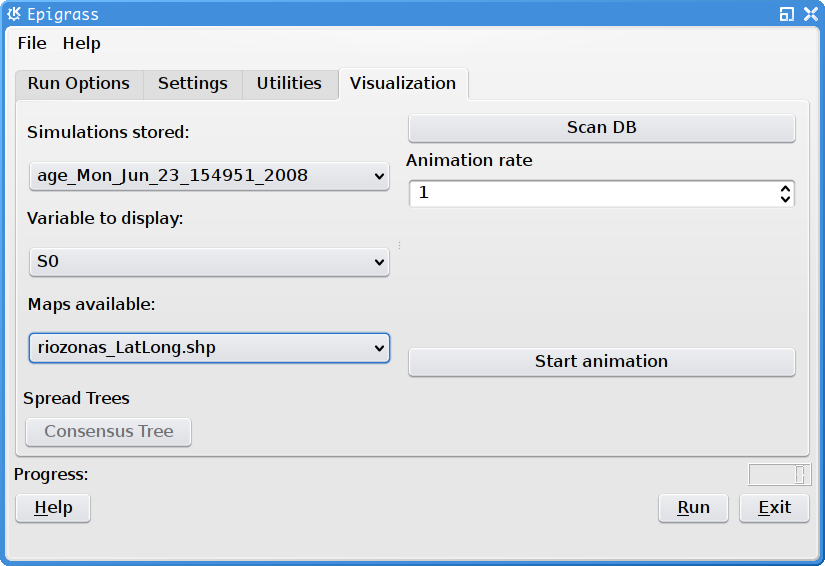
\includegraphics{epigrass4.png}
\caption{Visualization tab of the Epigrass GUI. The simulations and varibales to inspect are chosen here.}\end{figure}

Once the \emph{Start animation} button is pressed, a graphical display window pops up, and the simulation results will be displayed as a map or a graph (if no map was specified at the \code{.epg}). The animation can be replayed or moved to any timestep by dragging on the slider under the display widget. When the user moved the mouse over a polygon in the map(or node in the graph) its name and geocode appears as a tooltip. Polygons (nodes) can be selected with the mouse to display their full time series in the plot below the top display widget.
\begin{figure}[htbp]
\centering

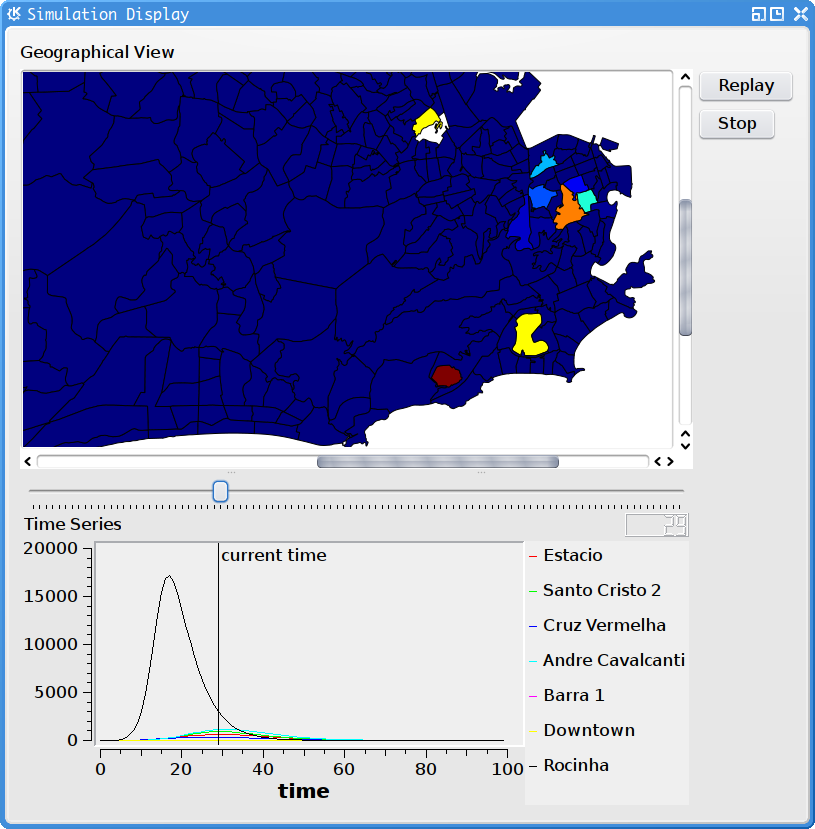
\includegraphics{simuview.png}
\end{figure}


\subsection{Operation}
\label{using:operation}
For running simulations, after all the information has been entered and checked on the first tab of the GUI, you can press the \emph{Run} button to start the simulation or the :guilabel{}`Exit{}` button. When the \emph{Run} button is pressed, the \code{\textasciitilde{}/.epigrassrc} file is updated with all the information entered in the GUI. If the \emph{Exit} button is pressed, all information entered since the last time the \emph{Run} button was pressed is lost.

Epigrass also allows running simulation straight from the command line, with the \textbf{epirunner} executable. all you have to do is:

\begin{Verbatim}[commandchars=\\\{\}]
\PYGZdl{} epirunner mymodel.epg
\end{Verbatim}

and the model will executed with the settings specified in the \code{\textasciitilde{}/.epigrassrc} file. for help with \emph{epirunner}, type:

\begin{Verbatim}[commandchars=\\\{\}]
\PYGZdl{} epirunner \PYGZhy{}h
Usage: epirunner [options] your\PYGZus{}model.epg

Options:
  \PYGZhy{}\PYGZhy{}version             show program\PYGZsq{}s version number and exit
  \PYGZhy{}h, \PYGZhy{}\PYGZhy{}help            show this help message and exit
  \PYGZhy{}b \PYGZlt{}mysql\textbar{}sqlite\textbar{}csv\PYGZgt{}, \PYGZhy{}\PYGZhy{}backend=\PYGZlt{}mysql\textbar{}sqlite\textbar{}csv\PYGZgt{}
                                                Define which datastorage backend to use
  \PYGZhy{}u DBUSER, \PYGZhy{}\PYGZhy{}dbusername=DBUSER
                                                MySQL user name
  \PYGZhy{}p DBPASS, \PYGZhy{}\PYGZhy{}password=DBPASS
                                                MySQL password for user
  \PYGZhy{}H DBHOST, \PYGZhy{}\PYGZhy{}dbhost=DBHOST
                                                MySQL hostname or IP address
\end{Verbatim}


\chapter{Analysis}
\label{analysis:id1}\label{analysis::doc}\label{analysis:analysis}

\chapter{Writing Custom Models}
\label{scripting::doc}\label{scripting:custom}\label{scripting:writing-custom-models}
\index{custom models}
The most powerful feature of Epigrass is the ability to use custom
models. It allows the user to specify intra-node dynamics and, in
doing so, break away from the limitations imposed by the built-in
models.

By learning to write his/her own models, the user begins to realize
the full potential of Epigrass, which goes beyond being a platform to
simulate networked epidemics. In reality Epigrass can be used to model
any distributed dynamical system taking place on a set of nodes
(connected or not).


\section{Getting Started}
\label{scripting:getting-started}
The best way to get started in writing custom models is to look at the
example distributed with Epigrass. It can be found in
\code{demos/CustomModel\_example.py}:

\begin{Verbatim}[commandchars=\\\{\}]
\PYG{c}{\PYGZsh{} This is a custom model to used in place of Epigrass\PYGZsq{} built\PYGZhy{}in models. Custom}
\PYG{c}{\PYGZsh{} models must always be on a file named CustomModel.py and contain at least}
\PYG{c}{\PYGZsh{} a function named Model. Both the File name and the function Names are case\PYGZhy{}sensitive,}
\PYG{c}{\PYGZsh{} so be careful. Please refer to the manual for intructions on how to write your}
\PYG{c}{\PYGZsh{} own custom models.}

\PYG{k}{def} \PYG{n+nf}{Model}\PYG{p}{(}\PYG{n+nb+bp}{self}\PYG{p}{,}\PYG{n+nb}{vars}\PYG{p}{,}\PYG{n}{par}\PYG{p}{,}\PYG{n}{theta}\PYG{o}{=}\PYG{l+m+mi}{0}\PYG{p}{,} \PYG{n}{npass}\PYG{o}{=}\PYG{l+m+mi}{0}\PYG{p}{)}\PYG{p}{:}
        \PYG{l+s+sd}{\PYGZdq{}\PYGZdq{}\PYGZdq{}}
\PYG{l+s+sd}{        Calculates the model SIR, and return its values.}
\PYG{l+s+sd}{        * vars The state variables of the models}
\PYG{l+s+sd}{        * par  The parameters (Beta, alpha, E,r,delta,B, w, p) see docs.}
\PYG{l+s+sd}{        * theta = infectious individuals from neighbor sites}
\PYG{l+s+sd}{        * npass = Total number of people arriving at this node}
\PYG{l+s+sd}{        \PYGZdq{}\PYGZdq{}\PYGZdq{}}
        \PYG{c}{\PYGZsh{} Get state variables\PYGZsq{} current values}

        \PYG{k}{if} \PYG{n+nb+bp}{self}\PYG{o}{.}\PYG{n}{parentSite}\PYG{o}{.}\PYG{n}{parentGraph}\PYG{o}{.}\PYG{n}{simstep} \PYG{o}{==} \PYG{l+m+mi}{1}\PYG{p}{:}  \PYG{c}{\PYGZsh{} if first step}
                \PYG{c}{\PYGZsh{} Define variable names to appear in the output}
                \PYG{n+nb+bp}{self}\PYG{o}{.}\PYG{n}{parentSite}\PYG{o}{.}\PYG{n}{vnames} \PYG{o}{=} \PYG{p}{(}\PYG{l+s}{\PYGZsq{}}\PYG{l+s}{Exposed}\PYG{l+s}{\PYGZsq{}}\PYG{p}{,}\PYG{l+s}{\PYGZsq{}}\PYG{l+s}{Infectious}\PYG{l+s}{\PYGZsq{}}\PYG{p}{,}\PYG{l+s}{\PYGZsq{}}\PYG{l+s}{Susceptible}\PYG{l+s}{\PYGZsq{}}\PYG{p}{)}
                \PYG{c}{\PYGZsh{} And get state variables\PYGZsq{}s initial values (stored in dict self.bi)}

                \PYG{n}{E}\PYG{p}{,}\PYG{n}{I}\PYG{p}{,}\PYG{n}{S} \PYG{o}{=} \PYG{p}{(}\PYG{n+nb+bp}{self}\PYG{o}{.}\PYG{n}{bi}\PYG{p}{[}\PYG{l+s}{\PYGZsq{}}\PYG{l+s}{e}\PYG{l+s}{\PYGZsq{}}\PYG{p}{]}\PYG{p}{,}\PYG{n+nb+bp}{self}\PYG{o}{.}\PYG{n}{bi}\PYG{p}{[}\PYG{l+s}{\PYGZsq{}}\PYG{l+s}{i}\PYG{l+s}{\PYGZsq{}}\PYG{p}{]}\PYG{p}{,}\PYG{n+nb+bp}{self}\PYG{o}{.}\PYG{n}{bi}\PYG{p}{[}\PYG{l+s}{\PYGZsq{}}\PYG{l+s}{s}\PYG{l+s}{\PYGZsq{}}\PYG{p}{]}\PYG{p}{)}
        \PYG{k}{else}\PYG{p}{:}   \PYG{c}{\PYGZsh{} if nor first step}
                \PYG{n}{E}\PYG{p}{,}\PYG{n}{I}\PYG{p}{,}\PYG{n}{S} \PYG{o}{=} \PYG{n+nb}{vars}

        \PYG{c}{\PYGZsh{} Get parameter values}
        \PYG{n}{N} \PYG{o}{=} \PYG{n+nb+bp}{self}\PYG{o}{.}\PYG{n}{parentSite}\PYG{o}{.}\PYG{n}{totpop}
        \PYG{n}{beta}\PYG{p}{,}\PYG{n}{alpha}\PYG{p}{,}\PYG{n}{e}\PYG{p}{,}\PYG{n}{r}\PYG{p}{,}\PYG{n}{delta}\PYG{p}{,}\PYG{n}{B}\PYG{p}{,}\PYG{n}{w}\PYG{p}{,}\PYG{n}{p} \PYG{o}{=} \PYG{p}{(}\PYG{n+nb+bp}{self}\PYG{o}{.}\PYG{n}{bp}\PYG{p}{[}\PYG{l+s}{\PYGZsq{}}\PYG{l+s}{beta}\PYG{l+s}{\PYGZsq{}}\PYG{p}{]}\PYG{p}{,}\PYG{n+nb+bp}{self}\PYG{o}{.}\PYG{n}{bp}\PYG{p}{[}\PYG{l+s}{\PYGZsq{}}\PYG{l+s}{alpha}\PYG{l+s}{\PYGZsq{}}\PYG{p}{]}\PYG{p}{,}
        \PYG{n+nb+bp}{self}\PYG{o}{.}\PYG{n}{bp}\PYG{p}{[}\PYG{l+s}{\PYGZsq{}}\PYG{l+s}{e}\PYG{l+s}{\PYGZsq{}}\PYG{p}{]}\PYG{p}{,}\PYG{n+nb+bp}{self}\PYG{o}{.}\PYG{n}{bp}\PYG{p}{[}\PYG{l+s}{\PYGZsq{}}\PYG{l+s}{r}\PYG{l+s}{\PYGZsq{}}\PYG{p}{]}\PYG{p}{,}\PYG{n+nb+bp}{self}\PYG{o}{.}\PYG{n}{bp}\PYG{p}{[}\PYG{l+s}{\PYGZsq{}}\PYG{l+s}{delta}\PYG{l+s}{\PYGZsq{}}\PYG{p}{]}\PYG{p}{,}\PYG{n+nb+bp}{self}\PYG{o}{.}\PYG{n}{bp}\PYG{p}{[}\PYG{l+s}{\PYGZsq{}}\PYG{l+s}{b}\PYG{l+s}{\PYGZsq{}}\PYG{p}{]}\PYG{p}{,}
        \PYG{n+nb+bp}{self}\PYG{o}{.}\PYG{n}{bp}\PYG{p}{[}\PYG{l+s}{\PYGZsq{}}\PYG{l+s}{w}\PYG{l+s}{\PYGZsq{}}\PYG{p}{]}\PYG{p}{,}\PYG{n+nb+bp}{self}\PYG{o}{.}\PYG{n}{bp}\PYG{p}{[}\PYG{l+s}{\PYGZsq{}}\PYG{l+s}{p}\PYG{l+s}{\PYGZsq{}}\PYG{p}{]}\PYG{p}{)}

        \PYG{c}{\PYGZsh{}Vacination event (optional)}
        \PYG{k}{if} \PYG{n+nb+bp}{self}\PYG{o}{.}\PYG{n}{parentSite}\PYG{o}{.}\PYG{n}{vaccineNow}\PYG{p}{:}
                \PYG{n}{S} \PYG{o}{\PYGZhy{}}\PYG{o}{=} \PYG{n+nb+bp}{self}\PYG{o}{.}\PYG{n}{parentSite}\PYG{o}{.}\PYG{n}{vaccov}\PYG{o}{*}\PYG{n}{S}

        \PYG{c}{\PYGZsh{} Model}
        \PYG{n}{Lpos} \PYG{o}{=} \PYG{n}{beta}\PYG{o}{*}\PYG{n}{S}\PYG{o}{*}\PYG{p}{(}\PYG{p}{(}\PYG{n}{I}\PYG{o}{+}\PYG{n}{theta}\PYG{p}{)}\PYG{o}{/}\PYG{p}{(}\PYG{n}{N}\PYG{o}{+}\PYG{n}{npass}\PYG{p}{)}\PYG{p}{)}\PYG{o}{*}\PYG{o}{*}\PYG{n}{alpha} \PYG{c}{\PYGZsh{}Number of new cases}
        \PYG{n}{Ipos} \PYG{o}{=} \PYG{p}{(}\PYG{l+m+mi}{1}\PYG{o}{\PYGZhy{}}\PYG{n}{r}\PYG{p}{)}\PYG{o}{*}\PYG{n}{I} \PYG{o}{+} \PYG{n}{Lpos}
        \PYG{n}{Spos} \PYG{o}{=} \PYG{n}{S} \PYG{o}{+} \PYG{n}{B} \PYG{o}{\PYGZhy{}} \PYG{n}{Lpos}
        \PYG{n}{Rpos} \PYG{o}{=} \PYG{n}{N}\PYG{o}{\PYGZhy{}}\PYG{p}{(}\PYG{n}{Spos}\PYG{o}{+}\PYG{n}{Ipos}\PYG{p}{)}

        \PYG{c}{\PYGZsh{} Update stats}
        \PYG{n+nb+bp}{self}\PYG{o}{.}\PYG{n}{parentSite}\PYG{o}{.}\PYG{n}{totalcases} \PYG{o}{+}\PYG{o}{=} \PYG{n}{Lpos} \PYG{c}{\PYGZsh{}update number of cases}
        \PYG{n+nb+bp}{self}\PYG{o}{.}\PYG{n}{parentSite}\PYG{o}{.}\PYG{n}{incidence}\PYG{o}{.}\PYG{n}{append}\PYG{p}{(}\PYG{n}{Lpos}\PYG{p}{)}

        \PYG{c}{\PYGZsh{} Raise site infected flag and add parent site to the epidemic history list.}
        \PYG{k}{if} \PYG{o+ow}{not} \PYG{n+nb+bp}{self}\PYG{o}{.}\PYG{n}{parentSite}\PYG{o}{.}\PYG{n}{infected}\PYG{p}{:}
                \PYG{k}{if} \PYG{n}{Lpos} \PYG{o}{\PYGZgt{}} \PYG{l+m+mi}{0}\PYG{p}{:}
                        \PYG{n+nb+bp}{self}\PYG{o}{.}\PYG{n}{parentSite}\PYG{o}{.}\PYG{n}{infected} \PYG{o}{=} \PYG{n+nb+bp}{self}\PYG{o}{.}\PYG{n}{parentSite}\PYG{o}{.}\PYG{n}{parentGraph}\PYG{o}{.}\PYG{n}{simstep}
                        \PYG{n+nb+bp}{self}\PYG{o}{.}\PYG{n}{parentSite}\PYG{o}{.}\PYG{n}{parentGraph}\PYG{o}{.}\PYG{n}{epipath}\PYG{o}{.}\PYG{n}{append}\PYG{p}{(}
                        \PYG{p}{(}\PYG{n+nb+bp}{self}\PYG{o}{.}\PYG{n}{parentSite}\PYG{o}{.}\PYG{n}{parentGraph}\PYG{o}{.}\PYG{n}{simstep}\PYG{p}{,}
                        \PYG{n+nb+bp}{self}\PYG{o}{.}\PYG{n}{parentSite}\PYG{p}{,}\PYG{n+nb+bp}{self}\PYG{o}{.}\PYG{n}{parentSite}\PYG{o}{.}\PYG{n}{infector}\PYG{p}{)}\PYG{p}{)}

        \PYG{n+nb+bp}{self}\PYG{o}{.}\PYG{n}{parentSite}\PYG{o}{.}\PYG{n}{migInf}\PYG{o}{.}\PYG{n}{append}\PYG{p}{(}\PYG{n}{Ipos}\PYG{p}{)}

        \PYG{k}{return} \PYG{p}{[}\PYG{l+m+mi}{0}\PYG{p}{,}\PYG{n}{Ipos}\PYG{p}{,}\PYG{n}{Spos}\PYG{p}{]}
\end{Verbatim}

Let's analyze the above code. The first thing to notice is that an Epigrass custom model is a Python program. So anything you can do with Python in your system, you can do in your custom model. Naturally, your knowledge of the Python programming language will define how far you can go in this customization. There are a few requirements on this Python program in order to make it a valid custom model from Epigrass's perspective.
\begin{enumerate}
\item {} \begin{description}
\item[{It must define a global function named \textbf{Model}. This function will be inserted as a method on every node object, at run time.}] \leavevmode\begin{enumerate}
\item {} \begin{description}
\item[{This function must declare the following arguments:}] \leavevmode\begin{itemize}
\item {} 
\emph{self}: reference to the model object.

\item {} 
\emph{vars}: A list with the values of the model's state variables in time t-1 in the same order as returned by this function.

\item {} 
\emph{par}: The parameters of the model. Listed in the same order as defined in the \code{.epg} file.

\item {} 
\emph{theta}: Number of infectious individuals arriving from neighboring sites. For disconnected models, it is 0.

\item {} 
\emph{npass}: The total number of passengers arriving from neighboring sites. For disconnected models, it is 0.

\end{itemize}

\end{description}

\item {} 
In the beginning of the function you define a list of strings (self.parentSite.vnames) which will be the names used when storing the resulting time-series in the database. Choose strings that are not very long and are meaningful. You only need to do this once, ate the beginning of the simulation so put it inside an \emph{if} statement, which will be executed only at time-step 1 (see code above).

\item {} 
After defining variable names, set their initial values in the same \emph{if} clause. An \emph{else} clause linked to this one will set variables values for the rest of the simulation.

\item {} 
Define local names for the total population \emph{N} and fixed parameters.

\item {} 
Proceed to implement your model anyway you see fit.

\item {} \begin{description}
\item[{Feed some site level variables (\emph{incidence},) with the result of the simulation.}] \leavevmode\begin{itemize}
\item {} 
\emph{incidence}: list of new cases per time step.

\item {} 
\emph{infected}: Boolean stating if the site has been infected, i.e., it has had an autoctonous case.

\item {} 
\emph{epipath}: This variable is at the graph level and contains the path of spread of the simulation.

\item {} 
\emph{migInf}: Number of infectious individuals in this site per time-step.

\end{itemize}

\end{description}

\item {} 
Finally, this function must return a list/tuple with the values of the state variables in the same order as received in vars.

\end{enumerate}

\end{description}

\end{enumerate}
\begin{quote}

\begin{notice}{warning}{Warning:}
The strings in self.parentSite.vnames must be valid \emph{SQL} variable names, or else you will have a insert error at the end of the simulation.
\end{notice}
\end{quote}

After defining this function with all its required features, you can continue to develop you custom model, writing other functions classes, etc. Note however, that only the \emph{Model} function will be called by Epigrass, so any other code you add to your program must be called from within that function.

\begin{notice}{note}{Note:}
Since \code{CustomModel} is imported from within Epigrass, any global code (unindented) in it is also  executed. So you may add imports and other initialization code.
\end{notice}

\begin{notice}{warning}{Warning:}
The name CustomModel.py is case-sensitive and cannot be changed. The same is true for the \emph{Model} function.
\end{notice}


\section{The Environment}
\label{scripting:the-environment}\begin{figure}[htbp]
\centering
\capstart

\includegraphics{Diagrama1.png}
\caption{Nesting of the objects inside a Simulate object.}\end{figure}

From quickly going through the example Custom model above it probably became clear, to the Python-initiated, that Yous can access variables at the node and graph levels.  This is possible because \emph{Model} becomes a method in a node object which in is turn is contained into a graph object (see figure).

Besides being nested within the \emph{graph} object, \emph{node} and \emph{edge} contain references to their containers. This means that using the introspective abilities of Python the user can access any information at any level of the full \emph{graph} model and use it in the custom model. In order to help you do this, Let's establish an API for developing custom models.


\subsection{Model Development API}
\label{scripting:model-development-api}
All attributes and methods (functions) from all around the simulation must be references from the model's  perspective, denoted by \emph{self}. The parent objects can be accessed through the following notation:
\begin{itemize}
\item {} \begin{description}
\item[{\emph{self.parentSite}}] \leavevmode
Is the Site (node) containing the model.

\end{description}

\item {} \begin{description}
\item[{\emph{self.parentSite.parentGraph}}] \leavevmode
Is the Graph containing the parent site of the model.

\end{description}

\end{itemize}

The following attributes and methods can be accessed by appending them to one one the objects above. For example:

\begin{Verbatim}[commandchars=\\\{\}]
\PYG{n+nb+bp}{self}\PYG{o}{.}\PYG{n}{parentSite}\PYG{o}{.}\PYG{n}{parentGraph}\PYG{o}{.}\PYG{n}{simstep}
\end{Verbatim}


\subsubsection{Site Attributes and Methods}
\label{scripting:site-attributes-and-methods}
Not all attributes and methods are listed, only the most useful. For a complete reference, look at the source code documentation.
\index{Site (built-in class)}

\begin{fulllineitems}
\phantomsection\label{scripting:Site}\pysigline{\strong{class }\bfcode{Site}}
self.parentSite. Actually named \emph{siteobj} in the source code.
\index{bi (Site attribute)}

\begin{fulllineitems}
\phantomsection\label{scripting:Site.bi}\pysigline{\bfcode{bi}}
Dictionary with initial values for all of the model's state variables. Keys are the variable names.

\end{fulllineitems}

\index{bp (Site attribute)}

\begin{fulllineitems}
\phantomsection\label{scripting:Site.bp}\pysigline{\bfcode{bp}}
Dictionary with initial values for all of the model's parameters. Keys are the parameter names.

\end{fulllineitems}

\index{totpop (Site attribute)}

\begin{fulllineitems}
\phantomsection\label{scripting:Site.totpop}\pysigline{\bfcode{totpop}}
Initial total population

\end{fulllineitems}

\index{ts (Site attribute)}

\begin{fulllineitems}
\phantomsection\label{scripting:Site.ts}\pysigline{\bfcode{ts}}
List containing the model output time series (variables in the same order of the model)

\end{fulllineitems}

\index{incidence (Site attribute)}

\begin{fulllineitems}
\phantomsection\label{scripting:Site.incidence}\pysigline{\bfcode{incidence}}
Incidence time series

\end{fulllineitems}

\index{infected (Site attribute)}

\begin{fulllineitems}
\phantomsection\label{scripting:Site.infected}\pysigline{\bfcode{infected}}
Has the site been already infected? (logical variable)

\end{fulllineitems}

\index{sitename (Site attribute)}

\begin{fulllineitems}
\phantomsection\label{scripting:Site.sitename}\pysigline{\bfcode{sitename}}
Site's name (provided in the .csv)

\end{fulllineitems}

\index{values (Site attribute)}

\begin{fulllineitems}
\phantomsection\label{scripting:Site.values}\pysigline{\bfcode{values}}
Tuple containing extra-variables provided by .csv file

\end{fulllineitems}

\index{parentGraph (Site attribute)}

\begin{fulllineitems}
\phantomsection\label{scripting:Site.parentGraph}\pysigline{\bfcode{parentGraph}}
Graph to which Site belongs (see class Graph)

\end{fulllineitems}

\index{edges (Site attribute)}

\begin{fulllineitems}
\phantomsection\label{scripting:Site.edges}\pysigline{\bfcode{edges}}
List containing all edge objects connected to Site

\end{fulllineitems}

\index{inedges (Site attribute)}

\begin{fulllineitems}
\phantomsection\label{scripting:Site.inedges}\pysigline{\bfcode{inedges}}
List containing all inbound edges

\end{fulllineitems}

\index{outedges (Site attribute)}

\begin{fulllineitems}
\phantomsection\label{scripting:Site.outedges}\pysigline{\bfcode{outedges}}
List containing all outbound edges

\end{fulllineitems}

\index{geocode (Site attribute)}

\begin{fulllineitems}
\phantomsection\label{scripting:Site.geocode}\pysigline{\bfcode{geocode}}
Site's geocode

\end{fulllineitems}

\index{modtype (Site attribute)}

\begin{fulllineitems}
\phantomsection\label{scripting:Site.modtype}\pysigline{\bfcode{modtype}}
Type of dynamic model running in Site

\end{fulllineitems}

\index{vaccination (Site attribute)}

\begin{fulllineitems}
\phantomsection\label{scripting:Site.vaccination}\pysigline{\bfcode{vaccination}}
Time and coverage of vaccination event. Format as in .epg

\end{fulllineitems}

\index{vaccineNow (Site attribute)}

\begin{fulllineitems}
\phantomsection\label{scripting:Site.vaccineNow}\pysigline{\bfcode{vaccineNow}}
Flag indicating that it is vaccine day (0 or 1)

\end{fulllineitems}

\index{vaccov (Site attribute)}

\begin{fulllineitems}
\phantomsection\label{scripting:Site.vaccov}\pysigline{\bfcode{vaccov}}
Current vaccination coverage

\end{fulllineitems}

\index{vaccinate() (Site method)}

\begin{fulllineitems}
\phantomsection\label{scripting:Site.vaccinate}\pysiglinewithargsret{\bfcode{vaccinate}}{\emph{cov}}{}
At time t, the population is vaccinated with coverage cov

\end{fulllineitems}

\index{getOutEdges() (Site method)}

\begin{fulllineitems}
\phantomsection\label{scripting:Site.getOutEdges}\pysiglinewithargsret{\bfcode{getOutEdges}}{}{}
Returns list of outbound edges

\end{fulllineitems}

\index{getInEdges() (Site method)}

\begin{fulllineitems}
\phantomsection\label{scripting:Site.getInEdges}\pysiglinewithargsret{\bfcode{getInEdges}}{}{}
Returns list of inbound edges

\end{fulllineitems}

\index{getNeighbors() (Site method)}

\begin{fulllineitems}
\phantomsection\label{scripting:Site.getNeighbors}\pysiglinewithargsret{\bfcode{getNeighbors}}{}{}
Returns a dictionary of neighbor sites as keys and distances as values

\end{fulllineitems}

\index{getDistanceFromNeighbor() (Site method)}

\begin{fulllineitems}
\phantomsection\label{scripting:Site.getDistanceFromNeighbor}\pysiglinewithargsret{\bfcode{getDistanceFromNeighbor}}{\emph{site}}{}
Returns the distance in km from a given neighbor

\end{fulllineitems}

\index{getDegree() (Site method)}

\begin{fulllineitems}
\phantomsection\label{scripting:Site.getDegree}\pysiglinewithargsret{\bfcode{getDegree}}{\emph{site}}{}
Returns degree of this site, that is, the number of sites connected to it

\end{fulllineitems}


\end{fulllineitems}



\subsubsection{Graph Attributes and Methods}
\label{scripting:graph-attributes-and-methods}
Not all attributes and methods are listed, only the most useful. For a complete reference, look at the source code documentation.
\index{Graph (built-in class)}

\begin{fulllineitems}
\phantomsection\label{scripting:Graph}\pysigline{\strong{class }\bfcode{Graph}}
self.parentSite.parentGraph
\index{simstep (Graph attribute)}

\begin{fulllineitems}
\phantomsection\label{scripting:Graph.simstep}\pysigline{\bfcode{simstep}}
Time-step of the simulation. Use it to keep track of the simulation progress.

\end{fulllineitems}

\index{speed (Graph attribute)}

\begin{fulllineitems}
\phantomsection\label{scripting:Graph.speed}\pysigline{\bfcode{speed}}
The speed of the transportation system

\end{fulllineitems}

\index{maxstep (Graph attribute)}

\begin{fulllineitems}
\phantomsection\label{scripting:Graph.maxstep}\pysigline{\bfcode{maxstep}}
Final time-step of the simulation

\end{fulllineitems}

\index{episize (Graph attribute)}

\begin{fulllineitems}
\phantomsection\label{scripting:Graph.episize}\pysigline{\bfcode{episize}}
Current size of the epidemic, graph-wise.

\end{fulllineitems}

\index{site\_list (Graph attribute)}

\begin{fulllineitems}
\phantomsection\label{scripting:Graph.site_list}\pysigline{\bfcode{site\_list}}
Full list of nodes in the graph. Each element in this list is a real node object.

\end{fulllineitems}

\index{edge\_list (Graph attribute)}

\begin{fulllineitems}
\phantomsection\label{scripting:Graph.edge_list}\pysigline{\bfcode{edge\_list}}
Full list of nodes in the graph. Each element in this list is a real node object.

\end{fulllineitems}

\index{getSite() (Graph method)}

\begin{fulllineitems}
\phantomsection\label{scripting:Graph.getSite}\pysiglinewithargsret{\bfcode{getSite}}{\emph{name}}{}
Returns an site object named \emph{name}

\end{fulllineitems}


\end{fulllineitems}



\chapter{Indices and tables}
\label{index:indices-and-tables}\begin{itemize}
\item {} 
\emph{genindex}

\item {} 
\emph{modindex}

\item {} 
\emph{search}

\end{itemize}



\renewcommand{\indexname}{Index}
\printindex
\end{document}
